%\documentclass[journal=jpccck,manuscript=article]{achemso}
%\usepackage[numbers,super]{natbib}
%
%\usepackage{graphicx}
%\usepackage{xcolor}
%\usepackage{todonotes}
%
%\def\ket#1{| #1 \rangle}
%\def\bra#1{\langle #1 |}
%
%\usepackage[utf8]{inputenc} % set input encoding (not needed with XeLaTeX)
%\usepackage{verbatim}
%\usepackage{amsfonts}
%\usepackage{graphicx}
%\newcommand{\overbar}[1]{\mkern 2.2mu\overline{\mkern-2.2mu#1\mkern-2.2mu}\mkern 2.2mu}
%\usepackage{multirow}
%\usepackage{array}
%\usepackage{varwidth}
%\usepackage{bm}
%
%\title{Frozen Virtual Natural Orbitals ++ for Coupled Cluster Linear-Response Theory}
%\author{Ashutosh Kumar}
%\affiliation{Department of Chemistry, Virginia Tech, Blacksburg, Virginia 24061, U.S.A.}
%\author{T.\ Daniel Crawford}
%\email{crawdad@vt.edu}
%\affiliation{Department of Chemistry, Virginia Tech, Blacksburg, Virginia 24061, U.S.A.}
%
%\date{\today}
%
%\begin{document}
%
%\begin{abstract} We present here the the modified frozen-virtual natural-orbital (NO) 
%approach, which we call FVNO++ for a compact representation of the 
%response of the coupled cluster wavefunction to external electric
%and magnectic fields. In our earlier work,\cite{Kumar17}
%we showed that the regular FVNO method performs rather poorly for 
%%The frozen-virtual natural-orbital (NO) approach, whereby the
%%unoccupied-orbital space is constructed using a correlated density such as
%%that from many-body perturbation theory, has proven to yield compact wave
%%functions for determining ground-state correlation energies and associated
%%properties, with corresponding occupation numbers providing a guide to the
%%truncation of the virtual space.  In this work this approach is tested for the
%%first time for the calculation of higher-order response properties,
%%particularly frequency-dependent dipole polarizabilities using coupled-cluster
%%theory.  We find that such properties are much more sensitive to the
%%truncation of virtual space in the natural orbital (NO) basis than in the
%%original canonical molecular orbital (CMO) basis, with truncation errors
%%increasing linearly with respect to the number of frozen virtual NOs.  The
%%reasons behind this poor performance include the more diffuse nature of NOs
%%with low occupation numbers as well as the reduction in sparsity of the
%%perturbed singles amplitudes in the NO basis and the neglect of orbital
%%response.  We tested a number of approaches
%%to improve the performance of the NO space, including the use of a
%%field-perturbed density to define the virtual orbitals and various
%%external-space corrections.  The truncation of the CMO space, on the other
%%hand, yields errors in coupled-cluster dipole polarizabilities of less than
%%2\% even after removing as much as 50\% of the full virtual space. We find
%%that this positive performance of the CMO space results from a cancellation of
%%errors due to the truncation of the unperturbed and perturbed amplitudes, as
%%well as sparsity of the singles amplitudes.  We introduce a simple criterion
%%called a dipole amplitude to use as a threshold for truncating the CMO basis
%%for such property calculations.  \end{abstract}
%\end{abstract}
%\maketitle

\section{Introduction}

One of the central problems limiting the application of accurate {\em ab
initio} methods like coupled-cluster (CC) theory to large molecular systems is their high 
computational cost, i.e., their computing and storage requirements 
exhibit polynomial scaling with the size of the system or equivalently
with the number of one electron basis functions used in these calculations.
Specifically, the size of the virtual space is of greater concern since  
they usually far outnumber the occupied orbitals. Furthermore, the canonical virtual orbitals
obtained from the Hartree-Fock (HF) procedure are non-local in nature and hence, 
the convergence of a determinantal expansion involving these orbitals
is quite slow. However, L{\"o}wdin \cite{Lowdin55}showed that using 
``natural orbitals'' (NOs) instead of the canonical HF orbitals can significantly 
accelerate the convergence of the configuration interaction (CI)
wavefunction expansion. The NOs are the eigenvectors of the 
one electron reduced density matrix (1-RDM) associated with a wavefunction. 
The corresponding eigenvalues are commonly referred to 
as ``occupation numbers''(ONs). Since L{\"o}wdin's pioneering 
work, NOs have found a lot of applications especially in techniques 
aimed at obtaining a compact representation of the virtual space for 
correlated calculations\cite{DePrince13,DePrince13:FNOs,Landau10,Sosa89,Taube05,Taube08}.
Please refer to ref.\cite{Landau10} for an excellent overview on this subject. 
Within the context of the CC theory, the frozen virtual NO (FVNO) scheme, where 
the NOs are usually obtained from the 1-RDM of a less expensive correlated method 
such as the second-order M{\"o}ller-Plesset (MP2) theory and the virtual space for subsequent 
CC calculations is truncated based on the values of the ONs has been used quite 
successfully to calculate correlation energies, 
ionization energies, etc. For example, Landau et al.\cite{Landau10} demonstrated 
that even after the removal of 70\% of the virtual space, the errors in
the ionization energies of the organic compounds under study were less than 1 kcal/mol.
However, it has been well established from previous studies that response 
properties are usually much more sensitive to the truncation of the wavefunction 
than simple energetics\cite{Korona04,Russ04,Russ08,McAlexander12,Friedrich15,McAlexander15:LRCC}. 
Recently, we investigated the applicability of such 
approaches for properties like dynamic polarizabilities using CC linear reponse theory
\cite{Koch90}. In contrast with the earlier studies\cite{Kumar17}, we got huge errors in polarizabilities 
which increased almost linearly with the number of truncated virtual orbitals. 
It was found that the ground-state MP2 density used to generate the NOs was 
unable to capture the response of the wavefunction to the external field. 
For example, the FVNO procedure threw out first the diffuse virtual 
orbitals, which are known to be very important to describe the low lying Rydberg type 
excited states (a common feature in majority of chiral compounds), 
resulting in large errors. This was not unsurprising since these diffuse 
orbitals have very low contributions to the correlation energy and hence 
possess very low occupation numbers. Consistent with the findings of Sundholm 
and co-workers\cite{Sundholm11}, dropping higher energy canonical HF 
virtual orbitals led to very small errors in polarizabilities due
to a) cancellation of errors resulting from the truncation of unperturbed 
and perturbed doubles amplitudes and b) the smaller magnitudes of the perturbed
singles amplitudes associated with such orbitals. 
We also constructed a first-order perturbed MP2 density by taking the gradient of the
ground state MP2 density with respect to the electric field, 
hoping that the ONs obtained from this density would be a better metric for 
estimating the importance of a virtual orbital 
for response properties but this approach only offered
minor improvements over the regular FVNO method. Nevertheless,
a suite of methods, conceptually not very different from our 
perturbed density approach have been proposed recently 
to calculate CC excitation energies. Baudin and co-workers 
used natural transition orbitals (NTOs) obtained from approximate 
CIS(D) transition densities in a scheme which they call CorNFLEx for 
calculating CC2 excitation energies of large solvated formamide 
clusters\cite{Baudin17}. In similar works, H{\"o}fener and Klopper 
obtained effective virtual spaces by combining MP2 
ground state density with excited state densities constructed from CIS 
excitation vectors\cite{HofenerKlopper17} while Mester {\em et al}. used MP2 and CIS(D) amplitudes 
to define their optimal virtual and occupied spaces\cite{Mester17,Mester18}.
These successful works prompted us to take back a closer look at the 
reasons behind the failure of our perturbed density approach. 
Finally, we have developed a new method which we call as FVNO++ 
where a second-order perturbed density is constructed to 
capture the response of the wavefunction to the external electric 
and magnetic fields. In this paper, we take a closer look at this 
scheme and report its performance in calculating CC dynamic 
polarizabilities and specific rotations of a number of chiral molecules.
%We also look at the potential applications of this approach to large
%solvated clusters.
\section{Theoretical Background}
\subsection{Coupled Cluster Response Theory}
The response functions for calculating dynamic higher-order properties 
can be defined by the frequency dependent coefficients appearing in the 
expansion of the expectation value of an appropriate time-independent 
operator in orders of the perturbation\cite{Koch90}.
\\
\begin{equation}
\begin{split}
\langle A \rangle (t) = \langle A \rangle + & \int_{-\infty}^{\infty}\
d\omega_1{\langle\langle A;V^{\omega_1}\rangle\rangle}_{\omega_1  \
+ i\alpha}e^{-i(\omega_1 + i\alpha)t} \\
& + \frac{1}{2} \int_{-\infty}^{\infty}d\omega_1\int_{-\infty}^{\infty}d\omega_2\
{\langle\langle A;V^{\omega_1};V^{\omega_2}\rangle\rangle}_{\omega_1 \
+ i\alpha,\omega_2 + i\alpha}e^{-i(\omega_1 + \omega_2 + 2i\alpha)t} + .....
\end{split}
\end{equation}
\\

%\begin{equation}
%A(t) = \langle \Psi^{(0)} | \hat{A} | \Psi^{(0)} \rangle \
%+ \langle \Psi^{(1)}(t) | \hat{A} | \Psi^{(0)} \rangle\
%+ \langle \Psi^{(0)} | \hat{A} | \Psi^{(1)}(t) \rangle\ 
%+ \langle \Psi^{(1)}(t) | \hat{A} | \Psi^{(1)}(t) \rangle + ... \\
%\end{equation}
Here $\langle A \rangle$ is the time independent expectation value and
${\langle\langle A;V^{\omega_1}\rangle\rangle}_{\omega_1 + i\alpha}$
%${\langle\langle A,V^{\omega_1},V^{\omega_2}\rangle\rangle}_{\omega_1 + i\alpha,\omega_2 + i\alpha}$ is the 
is the linear response function (LRF) i.e. the first order change in the expectation value of 
$A$ in a time-dependent field $V$ at frequency $\omega_1$. The third term in the expansion
contains the quadratic response function and so on. The CC-LRF is defined as,
\\
\begin{equation}
{\langle\langle A;B\rangle\rangle}_{\omega_1} =  \frac{1}{2}\hat{P}(A,B)[\langle 0 | \
[\hat{Y}^{B}_{\omega_1}, \bar{A}]|0\rangle + \langle 0 | \
(1 + \hat{\Lambda})|[\bar{A},\hat{X}^{B}_{\omega_1}]|0\rangle]
\end{equation}
\\
where $A$ and $B$ are the one electron perturbation operators,
$\hat{P}(A,B)$ simultaneously interchanges operators $A$ and $B$
and takes the complex conjugate of the expression,
$\omega_1$ is the frequency of the external field, 
$|0\rangle$ is the reference wavefunction, $\hat{\Lambda}$ is 
a linear de-excitation operator that parametrizes the CC left hand 
wavefunction to make sure that the CC gradients satisfy the 
generalized Hellman-Feynman theorem\cite{Koch90},
overbar on operataor $A$ denotes similarity transformation with the ground state
$T$ operator, $\bar{A} = e^{-\hat{T}}\hat{A}e^{\hat{T}}$
and $\hat{X}^{B}_{\omega_1}$ and $\hat{Y}^{B}_{\omega_1}$ are the excitation operators involving 
the first-order right and left hand perturbed amplitudes corresponding to operator 
$B$ respectively. These amplitudes can be obtained by solving a linear system
of equations,
\\
\begin{equation}
\begin{split}
&\sum_\nu\langle \mu | \big[(\bar{H} - \omega I),\tau_\nu\big] |0 \
\rangle X_{\nu}^{B} = -\langle \mu|\bar{B}|0 \rangle \\
&\sum_\nu Y_{\nu}^{B}\langle \nu | \big[(\bar{H} + \omega I),\tau_\mu\big] |0 \rangle \
+ \langle 0|(1 + \hat{\Lambda})|\big[\big[\bar{H},\tau_\nu\big],\tau_\mu\big] |0 \rangle\  X_{\nu}^{B}
= -\langle 0|(1 + \hat{\Lambda})|\big[\bar{B},\tau_\mu\big] |0 \rangle .\\
\end{split}
\end{equation}
\\
Here $\tau_\mu$, $\tau_\nu$ are the excitation operators which when acting on the
reference wavefunction $|0\rangle$ create excited determinats $|\mu\rangle$ 
and $|\nu\rangle$ respectively. Also, the dependence of perturbed amplitudes
 on $\omega_1$ is assumed. The right hand amplitudes are solved first after 
which they enter into the left hand amplitude equations as inhomogenous terms. 
It should be noted that these equations need to be solved for every cartesian 
component of the given perturbation operators. For example, calculation of 
optical rotation tensor using the length-gauge representation of the dipole 
operator would require solving a total of 12 linear equations, six each 
for both electric and magnetic dipole perturbation.
\subsection{Perturbed Natural Orbitals}
The CC-LRF (eq. 4.9) can also be formulated in terms of perturbed densities,
\\
\begin{equation}
{\langle\langle A;B\rangle\rangle}_{\omega_1} =  \frac{1}{2}\hat{P}(A,B)\big[\sum_{pq} A_{pq}[{D^{B^{\omega_1}}_{pq}}]^{(1)}\big]
\end{equation}
\\
where $[{D^{B^{\omega_1}}}]^{(1)}$ is the frequency dependent first-order
perturbed one-electron density related to operator B. The structures  
of the virtual-virtual blocks of perturbed densities of different orders
(for a given perturbation operator) can be easily identified in spin orbitals,
\\
\begin{equation}
\begin{split}
& D^{(0)}_{ab} = \frac{1}{2}(\lambda^{ij}_{ac})^{(0)}(t^{bc}_{ij})^{(0)} \
+ (\lambda^{i}_{a})^{(0)}(t^{b}_{i})^{(0)} \\
&D^{(1)}_{ab} = \frac{1}{2}[(\lambda^{ij}_{ac})^{(0)}(t^{bc}_{ij})^{(1)} \
+ (\lambda^{ij}_{ac})^{(1)}(t^{bc}_{ij})^{(0)}] + [(\lambda^{i}_{a})^{(0)}(t^{b}_{i})^{(1)}\
 + (\lambda^{i}_{a})^{(1)}(t^{b}_{i})^{(0)}] \\
&D^{(2)}_{ab} = \frac{1}{2}[{(\lambda^{ij}_{ac}})^{(1)}(t^{bc}_{ij})^{(1)}\
 + (\lambda^{ij}_{ac})^{(0)}(t^{bc}_{ij})^{(2)}]\ 
+ [(\lambda^{i}_{a})^{(1)} (t^{b}_{i})^{(1)} + (\lambda^{i}_{a})^{(0)}(t^{b}_{i})^{(2)}].\\
\end{split}
\end{equation}
\\
In the above equation, the indices $i,j$ and $a,b,c$ refer to occupied and virtual orbitals respectively
and Einstein summation notation is used. The first order perturbed amplitudes $(\lambda^{ij}_{ac})^{(1)}$ 
and $(t^{bc}_{ij})^{(1)}$ are nothing but the $\hat{X}^{B}_{\omega_1}$ and $\hat{Y}^{B}_{\omega_1}$ 
amplitudes that we saw earlier.\\ Just as the ground state MP2 density can transfer its knowledge of 
the electron correlation effects to the one electron basis (virtual NOs) through diagonalization, 
the perturbed densities can be used in a similar way to construct a compact ``perturbation aware''
basis. In our earlier work, we constructed a guess first-order perturbed density associated  
with each cartesian component (x,y,z) of the perturbation operator (dipole in the case of polarizabilities)
from MP2 amplitudes, took an average of the three densities and then diagonalized it to obtain our 
virtual space, but this approach offered only a minor improvement\cite{Kumar17}.
To investigate the reason behind the failure of this model, we constructed the virtual-virtual
block of the full CCSD first-order perturbed density. All the diagonal elements of this density 
matrix were found to be zeros irrespective of the perturbation operator. The exact reason for this
is not yet understood but clearly, the virtual NOs (VNOs) obtained from this (or guess) density 
do not carry any useful information. However, since the polarizabilities and specific rotations are 
of second-order in perturbation, we realized that second-order perturbed densities should in principle be a better 
metric for estimating the importance of a VNO for these properties.
In this paper, we use an average of second-order guess densities corresponding to each cartesian
component of an appropriate perturbation operator to define our virtual space 
for correlated response calculations. For a perturbation operator A, this guess density looks like:
\\
\begin{equation}
[{D^A_{ab}}]^{(2)} = \frac{1}{2}[t^{ac}_{ij}(A)]^{(1)}[t^{bc}_{ij}(A)]^{(1)} \
+ [t^{a}_{i}(A)]^{(1)} [t^{b}_{i}(A)]^{(1)}.
\end{equation}
where
\begin{equation}
\begin{split}
& t^{ac}_{ij}(A)^{(1)} = \frac{\bar{A}^{ac}_{ij}}{\overbar{H}_{aa} + \overbar{H}_{cc} - \overbar{H}_{ii} - \overbar{H}_{jj}},\\
& t^{a}_{i}(A)^{(1)} = \frac{\bar{A}^{a}_{i}}{\overbar{H}_{aa} - \overbar{H}_{ii}}.\\
\end{split}
\end{equation}
\\
and %Here, we have used MP2 amplitudes for the similarity transformation
\begin{equation}
\begin{split}
& \overbar{A}^{ac}_{ij} = P_{ij}^{ac}(t^{ec}_{ij}A^a_e - t^{ac}_{mj}A^m_i) ,\\
& \overbar{H}_{ii} =  f_{ii} + t^{ef}_{in}(2 \langle in|ef \rangle - \langle in|fe \rangle),\\
& \overbar{H}_{aa} =  f_{aa} - t^{fa}_{mn}(2 \langle mn|fa \rangle - \langle mn|af \rangle), \\
\end{split}
\end{equation}
\\
where $f$ refers to the Fock matrix. The above equations are derived by 
using the MP2 amplitudes for the similarity transformation, ignoring the terms 
involving second-order perturbed amplitudes and approximating the first-order 
perturbed $\lambda$ amplitudes with the corresponding $t$ amplitudes. 
The structure of the guess density chosen above becomes clearer 
if one looks at the equations for solving the first-order right-hand perturbed amplitudes 
(eq. 4.3) in terms of the inverse of the CC Jacobian,
\\
\begin{equation}
\begin{split}
& t^{ac}_{ij}(A)^{(1)}(\omega_1) = \sum_\mu - \langle\Phi_{ij}^{ac}| {(\bar{H} -\omega_1 I)}^{-1} |
\mu\rangle\langle \mu| \bar{A} | 0\rangle, \\
& t^{a}_{i}(A)^{(1)}(\omega_1) = \sum_\mu -\langle\Phi_{i}^{a}| {(\bar{H} -\omega_1 I)}^{-1} |
\mu\rangle \langle \mu| \bar{A} | 0\rangle \\
\end{split}
\end{equation}
\\
It can be easily seen that the guesses for $t^{ac}_{ij}(A)^{(1)}$ and 
$t^{a}_{i}(A)^{(1)}$ amplitudes in this work have been chosen by 
only considering the diagonal elements of $(\bar{H} -\omega_1 I)^{-1}$
matrix, which can be justified due to the diagonally dominant nature of the
$\bar{H}$ matrix. Furthermore, we keep $\omega_1$ as zero as we 
want to use the same density matrix for a given property calculation at different
frequencies. We also assume that removing $\omega_1$ should not significantly change the 
sparsity pattern of the perturbed amplitudes. \\
Finally, the basic outline of this approach
involves doing an MP2 calculation, generation of guess densities using MP2 amplitudes and 
perturbation operators, diagonalization of the virtual-virtual block of the guess density 
to obtain VNOs, truncation of VNOs with occupation numbers below a given threshold, 
diagonalization of the Fock matrix in the truncated VNO basis to obtain a semi-canonical 
basis, transformation of all the one and two electron integrals to this semi-canonical 
basis, followed by CCSD-LR calculations at given frequencies.
\section{Computational Details}
The main target of this work is large scale CC2\cite{Christiansen95:CC2}/CCSD calculations of specific 
rotations of solvated molecular clusters. However, first, we need to ensure 
that the FVNO++ approach has the right convergence behavior towards the full
canonical result. In this regard, we carry out dynamic polarizabilities 
and specific rotation calculations on linear chiral systems like 
hydrogen peroxide and hydrogen dimer (P)-($H_2)_n$ helices as they provide a 
convenient model for estimating the efficiency of these truncation schemes. 
%chiral molecules ranging from linear hydrogen peroxide, hydrogen dimer (P)-($H_2)_n$ 
%helices and (M)-1-Fluoralkanes to (S)-1-Phenylethanol, a molecule having two-dimensional 
%structure and ultimately molecules with cagelike structutes: (1R,4R)-Norbornenone
%and (1R,5R)-$\beta$-Pinene. 
\subsection{Polarizabilities}
Polarizability calculations on these chiral molecules can mostly be as seen as a diagnostic 
tool for gaining an insight into the nature of specific rotation calculations as one 
truncates the virtual space. Even though the response functions of both the properties 
are quite similar, polarizabilities are much less sensitive to the 
wavefunction truncation. However, the results on polarizabilities obtained in this work
can be extended to non-chiral systems as well. In all these calculations, the length-gauge 
(LG) representation of the electric dipole operator was used. The natural choice of 
the perturbed densities for such calculations would be $\sum\limits_q \frac{1}{3}[{D^{\mu_q}_{ab}}]^{(2)}$,
where $q \equiv [x,y,z]$ . 
\subsection{Specific Rotations}
All the specific rotation calculations in this work employ the LG representation.
%, the LG representation is again employed
%For the specific rotation calculations, we again employ the LG 
%and modified velocity gauge (MVG)\cite{Pedersen04} 
%representation 
Even though LG specific rotations are dependent on the choice of origin for the CC2/CCSD-LR method,
they are a good starting point for our analysis as they show a faster convergence towards the CBS 
(complete basis set) limit than the velocity gauge (VG) representation. Since these calculations 
involve both electric and magnetic dipole operators, we use, in addition to the electric dipole 
based densities, i.e. FVNO++ ($\mu$), two other approaches of defining our virtual space.
The first approach, FVNO++ ($\mu*L$) builds the density as a product of the first order amplitudes corresponding
to the electric and magnetic perturbations ($L$). However, this makes the density matrix non-positive 
definite and both positive and negative eigenvalues appear as a result. Nevertheless, we truncate 
these ``VNOs" based on the absolute values of their ``ONs". The second approach, FVNO++ ($\mu,L$) builds two truncated VNO 
spaces (50\% in this work) based on the densities of the electric and magnetic dipole operators individually and does a singular 
value decomposition on the union of the two spaces. Finally, just like before, the VNOs are truncated based on their singular values.
We report the performance of all three approaches in this work.
%
%choice of how to construct these perturbed densities. Both $[{D^{\mu_q}_{ab}}]^{(2)}$ 
%and $[{D^{m_q}_{ab}}]^{(2)}$ seem to be valid choices. Hence, in this work, we report the performance
%of three approaches for defining the virtual space for specific rotation calculations.
%
%
%However, premilinary results obtained using 
%magnetic dipole based perturbed densities 
% Hence, we use both the densities
%for defining our virtual space and compare their performances.
%Another possible option is to diagonalize both the densities separately, truncate the VNOs,
%and then form the virtual space by taking a union of the truncated VNOs. 
%Similarly, in MVG calculations, we use both $[{D^{p_q}_{ab}}]^{(2)}$ 
%and $[{D^{m_q}_{ab}}]^{(2)}$ as our definitions of 
%perturbed densities where $p$ is the momentum operator, i.e. 
%$p_q = -i\frac{\partial}{\partial{q}}$. 
%We report the performances of both the three approaches for specific rotations.\\ \\
The primary basis set used in this work is aug-cc-pVDZ\cite{Dunning89,Kendall92,Woon94}
and all the property calculations were carried out at 589 nm using 
using Psi4 and Psi4Numpy software packages.\cite{Parrish17, Smith18}
%We also report the sparsity pattern of the guess densities of large
%solvated molecular clusters using DF-MP2 which give us an estimate of 
%the computational savings that can be exploited for such systems. 
It should be noted that we have used the same virtual space for calculating both unperturbed
and perturbed amplitudes as this ensures a match with results obtained from
the finite-field procedures. The use of only perturbed densities for solving 
both unperturbed and perturbed amplitudes can be justified due to an inherent
insensitiviy of these response properties to the values of the ground state amplitudes.
For example, Table ~\ref{cclr_justify} shows that the values of specific rotations and polarizabilities 
obtained using the CCSD-LR(1) scheme which involves only one iteration of the CCSD $\hat{T}$ equation while 
approximating the $\lambda_\mu$ amplitudes with the corresponding $t_\mu$ amplitudes, are very close to 
the full canonical result (CCSD-LR).
 \begin{table}[h]
 \caption{{\footnotesize Comparison of the canonical CCSD-LR polarizabilities in atomic units ($\alpha$) and specific rotations ($[\alpha]$) in deg $\text{dm}^{−1}$(g/mL)$^{−1}$ of different test cases calculated at 589 nm with that of the approximated CCSD-LR(1) scheme.}}
%\begin{table}[h]
\centering
\begin{tabular}{lllll}
\hline
 & \multicolumn{2}{c}{CCSD-LR(1)} & \multicolumn{2}{c}{CCSD-LR} \\
%\hline{2-8} 
\cline{2-5}
 Molecules & $\alpha$ & $[\alpha]$ & $\alpha$ & $[\alpha]$ \\ % Column names row
\hline
H$_2$O$_2$  & 14.2 & -175.3 &  14.2 &  -185.5   \\
\hline
(H$_2$)$_4$ & 19.6 & 1357.9 &  19.3 &  1322.9 \\
\hline
(H$_2$)$_5$ & 24.1  & 1409.3 & 23.8 &  1380.6  \\
\hline
(H$_2$)$_6$ & 28.7 & 1542.7 & 28.2 &   1508.8 \\
\hline
(H$_2$)$_7$ & 33.0 & 1643.0 & 32.5 &   1606.3  \\
\hline
\\
\end{tabular}
%\caption{Specific rotations in (deg dm$^{\text{-1}}$(g/mL)$^{\text{-1}}$) for solvated structures.}
\label{cclr_justify}
\end{table}
%\begin{center}
% \begin{tabular}{ccc}
% Molecule & CCSD-LR(1) & CCSD-LR(2) \\ \hline
% H$_2$O$_2$ & 1 & 2 \\
% (H$_2$)$_4$ & 2 & 4 \\ 
% (H$_2$)$_5$ & 2 & 4 \\
% (H$_2$)$_6$ & 2 & 4 \\
% (H$_2$)$_7$ & 2 & 4 \\ 
% \end{tabular}
%\end{center}
% \end{table}
\section{Results and Discussion}
We demonstrated the importance of diffuse virtual orbitals for calculating  
dynamic polarizabilities of hydrozen peroxide in our previous work.
Thus, a better approach for calculating response properties with natural
orbitals would be to preserve these diffuse orbitals and apply the FVNO procedure 
to the ``non-diffuse" virtual space only where the orbital spatial extent (OSE), 
$\langle\phi_a| r^2 | \phi_a\rangle$, can be taken as a measure of the diffusivity 
of a virtual orbital ($\phi_a)$. Hence, we sorted the virtual canonical MOs 
according to their OSEs and chose an empirical cutoff that that led to the 
retention of the 26 most diffuse orbitals for the H$_2$O$_2$ molecule in the
aDZ basis. The MP2 ground stare density matrix is then created and diagonalized in the 
remaining (29) virtual space and the VNOs with low ONs are removed one by one. We refer 
to this modified FVNO scheme as FVNO(M). Fig.~\ref{fig:fvno(m)_h2o2_adz_polar_optrot} %and ~\ref{fig:fvno(m)_optrot}
\begin{figure}
\begin{subfigure}{.5\textwidth}
  \centering
  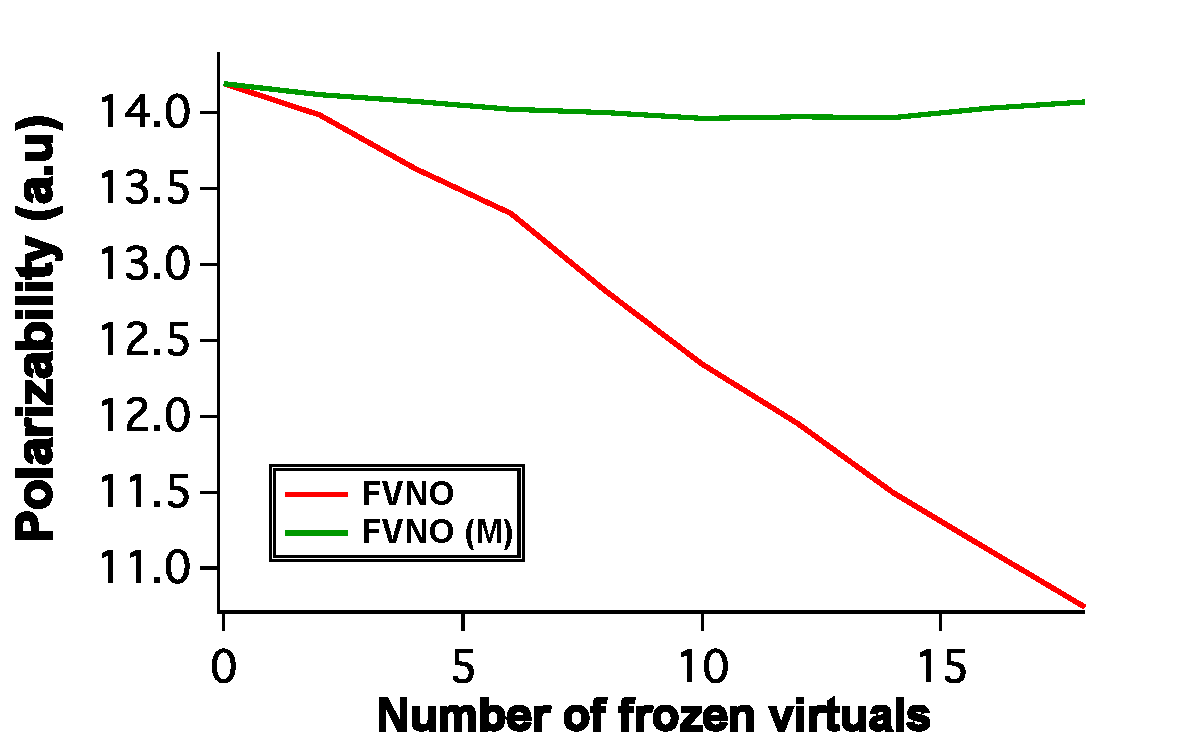
\includegraphics[width=.9\linewidth]{figures_fvno++/fvno(m)_h2o2_adz_polar.pdf}
  \caption{}
  \label{fig:sfig1}
\end{subfigure}%
\begin{subfigure}{.5\textwidth}
  \centering
  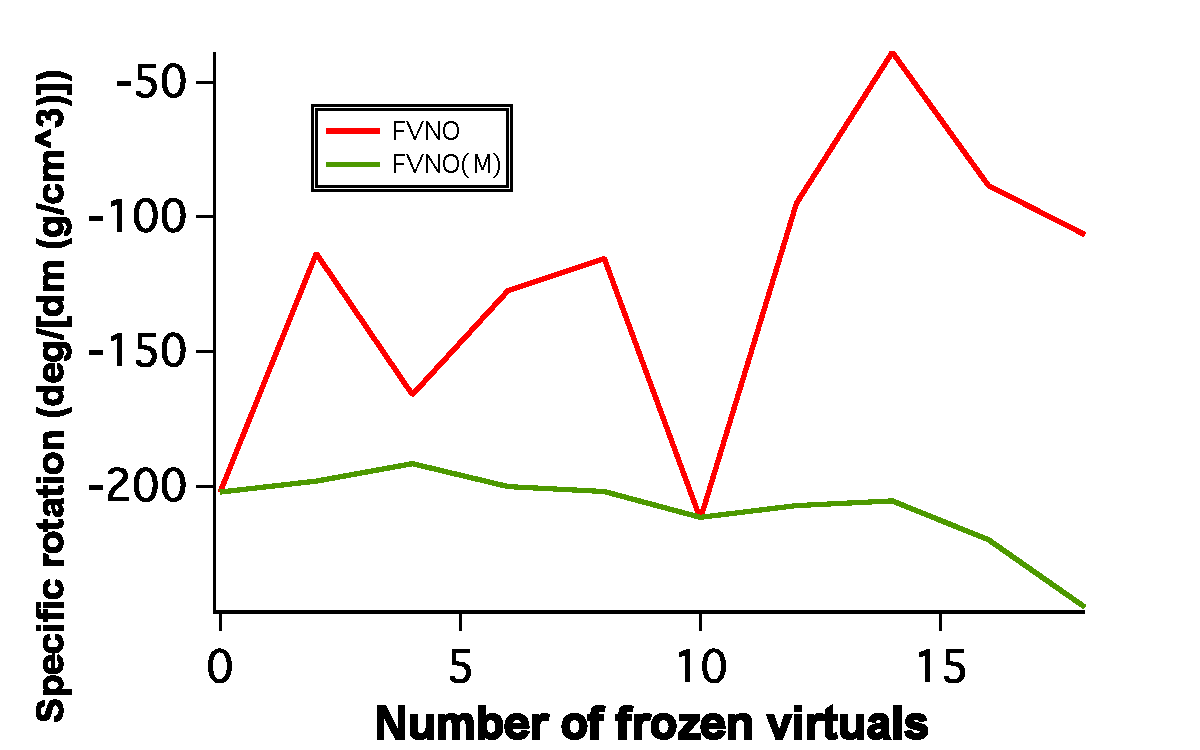
\includegraphics[width=.9\linewidth]{figures_fvno++/fvno(m)_h2o2_adz_optrot.pdf}
  \caption{}
  \label{fig:sfig2}
\end{subfigure}
\caption{{\footnotesize CCSD/aDZ polarizabilities (a) and specific rotations (b) of H$_2$O$_2$ in both FVNO and FVNO(M) schemes as a function of
the number of virtual orbitals removed.}}
\label{fig:fvno(m)_h2o2_adz_polar_optrot}
\end{figure}
%\begin{MyFigure}[h!]
%\centering
%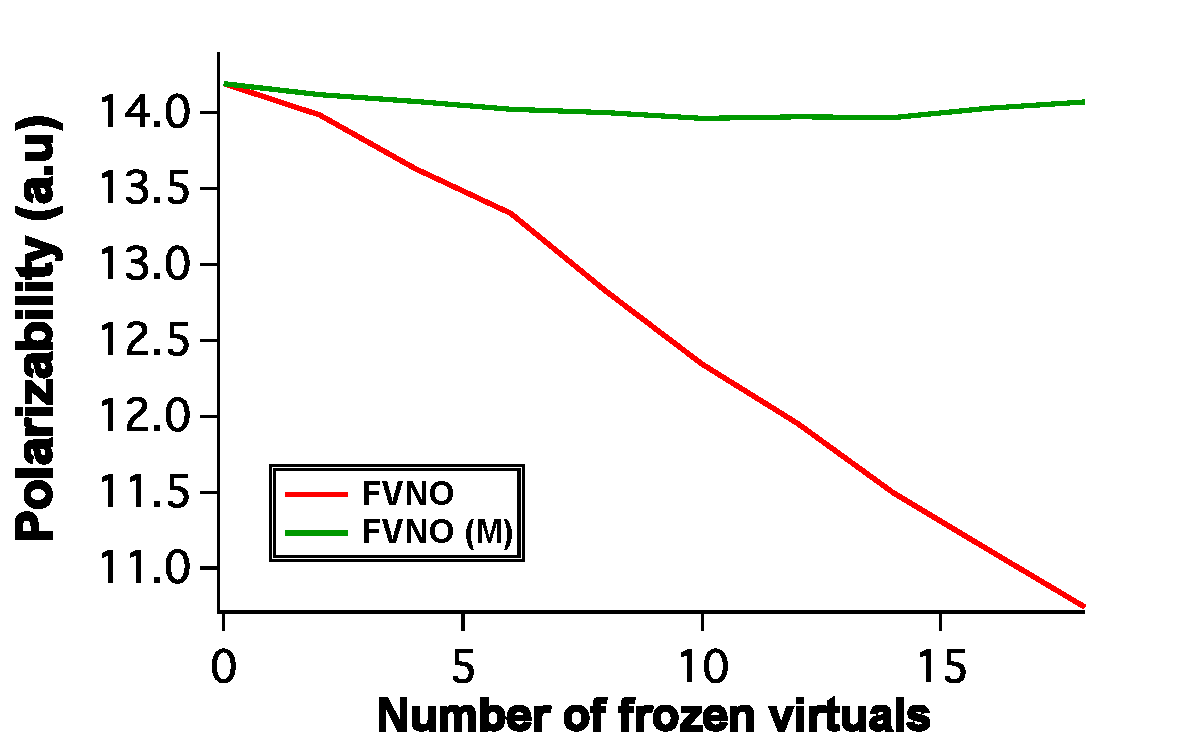
\includegraphics[width=0.5\linewidth]{figures_fvno++/fvno(m)_h2o2_adz_polar.pdf}
%\caption{{\footnotesize CCSD/aDZ polarizabilities of
%H$_2$O$_2$ in both FVNO and FVNO(M) schemes as a function of 
%number of virtual orbitals removed.}}
%\label{fig:fvno(m)_polar}
%\end{MyFigure}
%\begin{MyFigure}[h!]
%\centering
%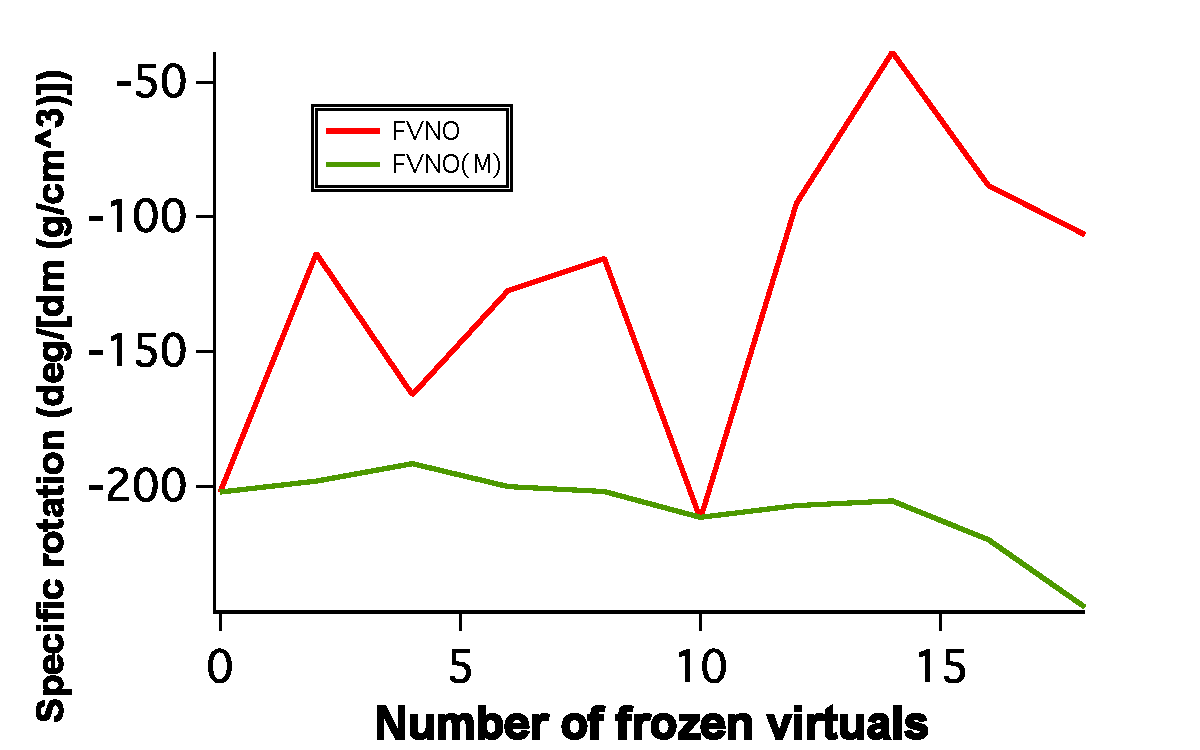
\includegraphics[width=0.5\linewidth]{figures_fvno++/fvno(m)_h2o2_adz_optrot.pdf}
%\caption{{\footnotesize CCSD/aDZ/MVG specific rotations of
%H$_2$O$_2$ in both FVNO and FVNO(M) schemes as a function of 
%number of virtual orbitals removed.}}
%\label{fig:fvno(m)_optrot}
%\end{MyFigure}
compares the performances of both the approaches for calculating CCSD dynamic polarizabilities and specific rotations 
%using the modified velocity gauge (MVG) representation\cite{Pedersen04} 
of the H$_2$O$_2$/aDZ system at 589 nm. Unsurprisingly, the errors in the FVNO(M) scheme are minimal compared to the original scheme for 
both polarizabilities and specific rotations even after 18 (out of 29) ``non-diffuse" VNOs are removed.
Specifically, the specific rotations curves are much well behaved in the 
FVNO(M) approach. Similar trends can be observed for other excited state
properties like excitation energies, oscillator strengths and rotational 
strengths as well. Figure ~\ref{fig:fvno(m)_h2o2_adz_ee_rs} plots the EOM-CCSD 
excitation energies and rotational strengths for the lowest four excited states of the H$_2$O$_2$/aDZ system
in both FVNO and FVNO(M) procedures as a function of the number of virtual orbitals removed.
\begin{figure}
\begin{subfigure}{.5\textwidth}
  \centering
  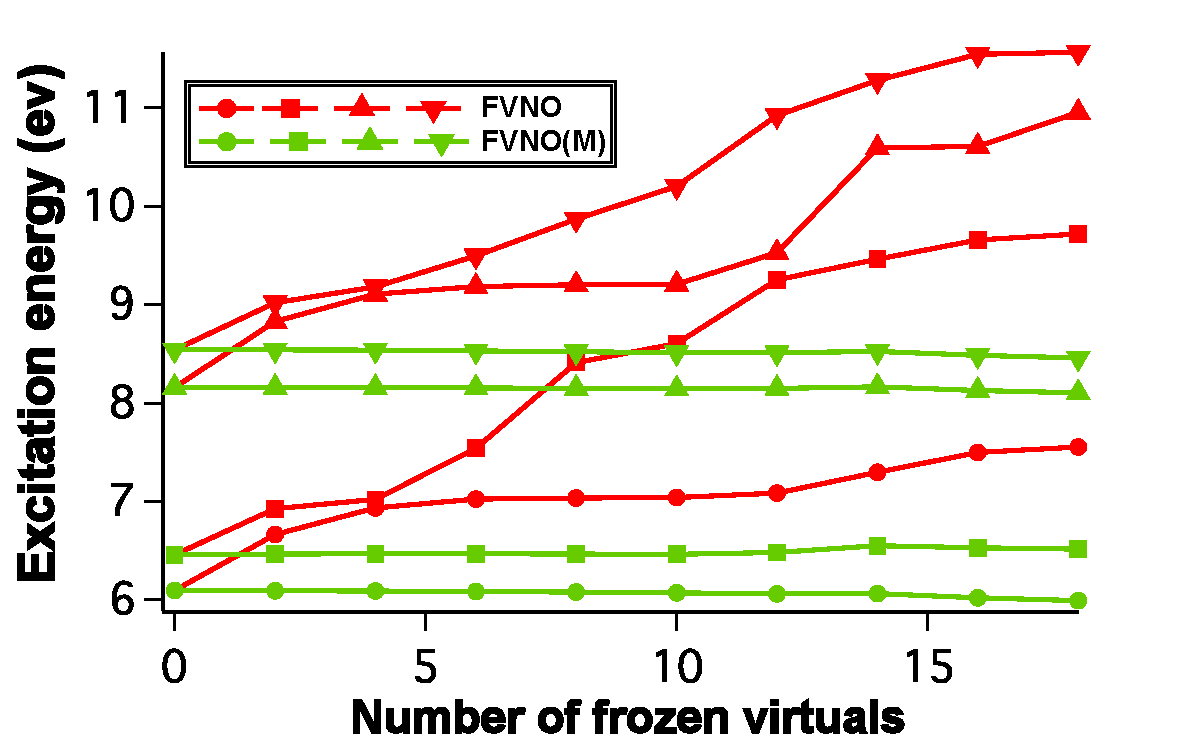
\includegraphics[width=.9\linewidth]{figures_fvno++/fvno(m)_h2o2_adz_ee.pdf}
  \caption{}
  \label{fig:sfig1}
\end{subfigure}%
\begin{subfigure}{.5\textwidth}
  \centering
  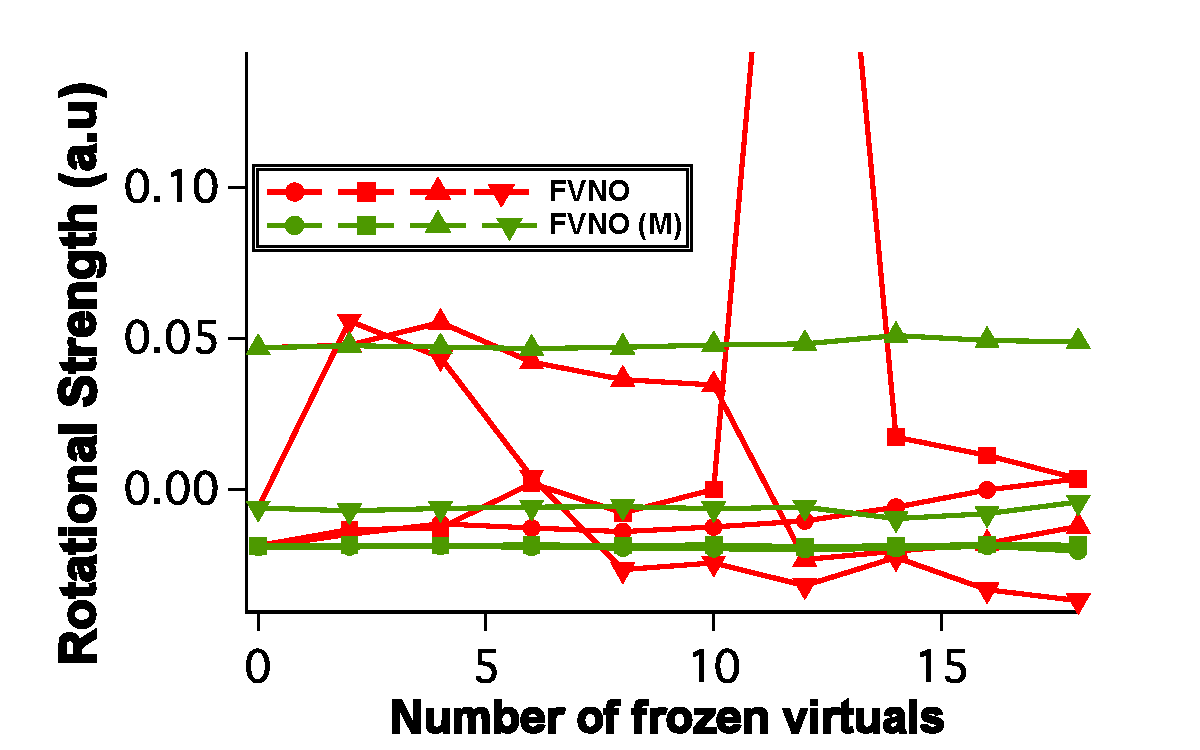
\includegraphics[width=.9\linewidth]{figures_fvno++/fvno(m)_h2o2_adz_rs.pdf}
  \caption{}
  \label{fig:sfig2}
\end{subfigure}
\caption{{\footnotesize EOM-CCSD/aDZ excitation energies (a) and rotational strengths (b) of the lowest four excited states of H$_2$O$_2$ in both FVNO and FVNO(M) schemes as a function of the number of virtual orbitals removed.}}
\label{fig:fvno(m)_h2o2_adz_ee_rs}
\end{figure}
%\begin{MyFigure}[h!]
%\centering
%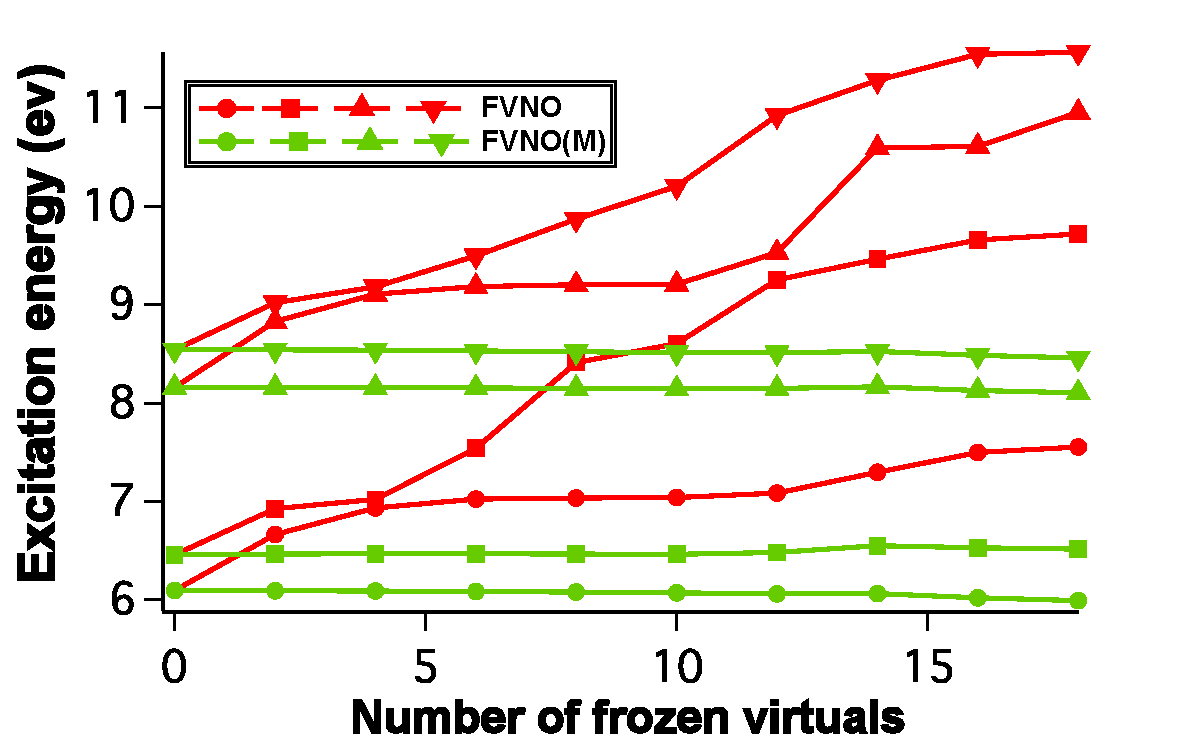
\includegraphics[width=0.6\linewidth]{figures_fvno++/fvno(m)_h2o2_adz_ee.pdf}
%\caption{{\footnotesize EOM-CCSD/aDZ excitation energies of the lowest four excited states of H$_2$O$_2$ in both FVNO and FVNO(M) schemes as a function of the number of virtual orbitals removed.}}
%\label{fig:fvno(m)_ee}
%\end{MyFigure}
It can be easily observed that the FVNO(M) curve is very well-behaved for 
both the properties for all the four states and the errors in excitation energies 
are less than 0.1 eV even after removing as much as 18 virtual orbitals i.e. 33 \% of the virtual
space. The rotational strengths also see a drastic improvement in the FVNO(M) scheme,
(especially the second lowest excited state).
%One can see the exact same trend in the case of rotational strengths
%as well.
%in figures ~\ref{fig:fvno(m)_os} and 
%~\ref{fig:fvno(m)_rs} which plot oscillator and rotational strengths respectively.
%\begin{MyFigure}[h!]
%\centering
%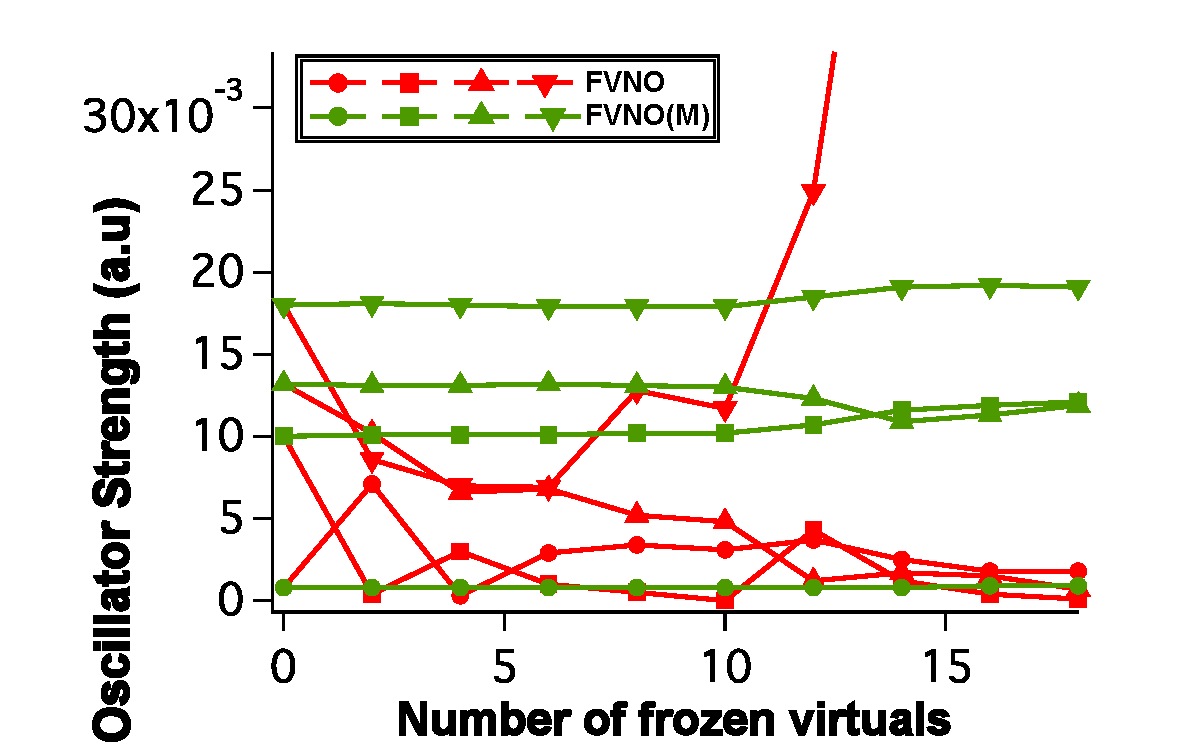
\includegraphics[width=0.6\linewidth]{figures_fvno++/fvno(m)_h2o2_adz_os.pdf}
%\caption{{\footnotesize EOM-CCSD/aDZ oscillator strengths of the lowest four excited states of H$_2$O$_2$ in both FVNO and FVNO(M) schemes as a function of the number of virtual orbitals removed.}}
%\label{fig:fvno(m)_os}
%\end{MyFigure}
%\begin{MyFigure}[h!]
%\centering
%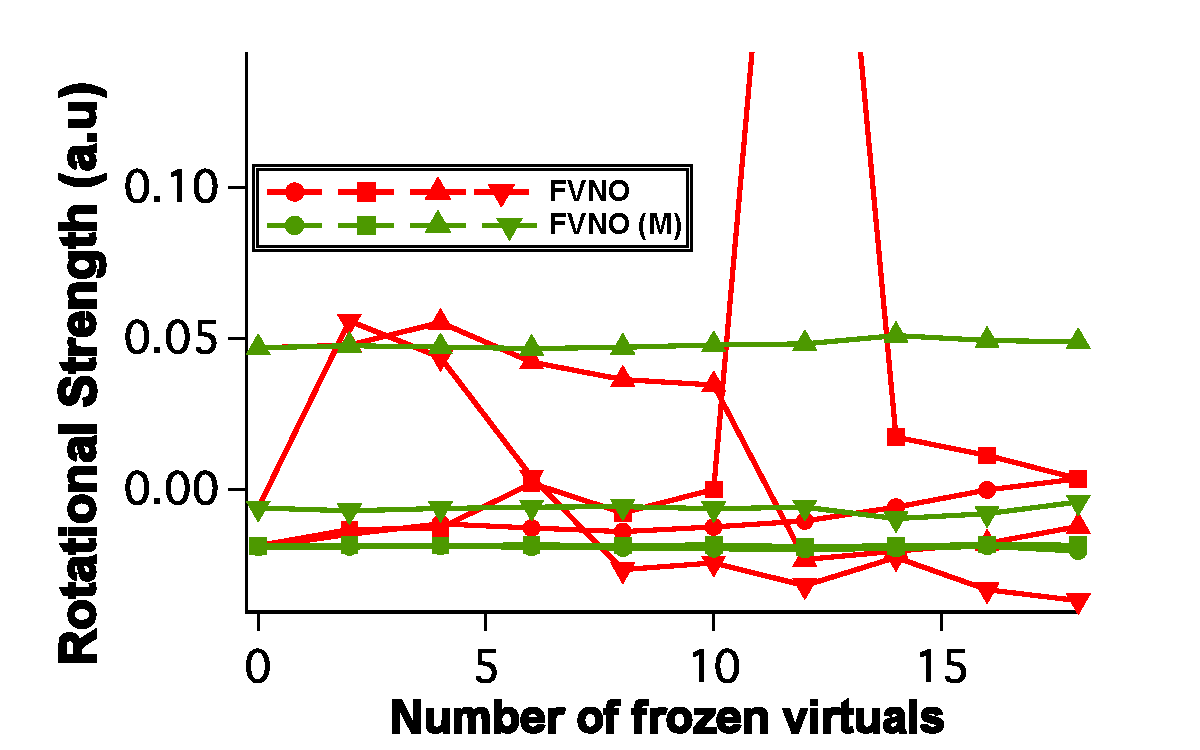
\includegraphics[width=0.6\linewidth]{figures_fvno++/fvno(m)_h2o2_adz_rs.pdf}
%\caption{{\footnotesize EOM-CCSD/aDZ rotational strengths of the lowest four excited states of H$_2$O$_2$ in both FVNO and FVNO(M) schemes as a function of the number of virtual orbitals removed.}}
%\label{fig:fvno(m)_rs}
%\end{MyFigure}
It should be noted that similar results can be expected for a majority of chiral molecules who 
like hydrogen peroxide require diffuse orbitals for a better description of the
Rydberg states. However, extension of this method to larger systems is not 
straightforward as OSEs are not a very robust crietria for the selction of diffuse 
orbitals. Furthermore, not all diffuse orbitals are equally important for 
calculating these response properties. The FVNO++ scheme on the other hand has a very well-defined 
truncation criteria based on ONs and the structure of the perturbed density used in this 
approach closely resembles the response functions used to calculate these 
properties. Thus, the FVNO++ approach, by construction, should mimic the performance of the FVNO(M)
scheme as seen above. Fig.~\ref{fig:fvno++_h2o2_adz_polar_optrot_lg} 
%\begin{figure}
%\begin{subfigure}{.5\textwidth}
%  \centering
%  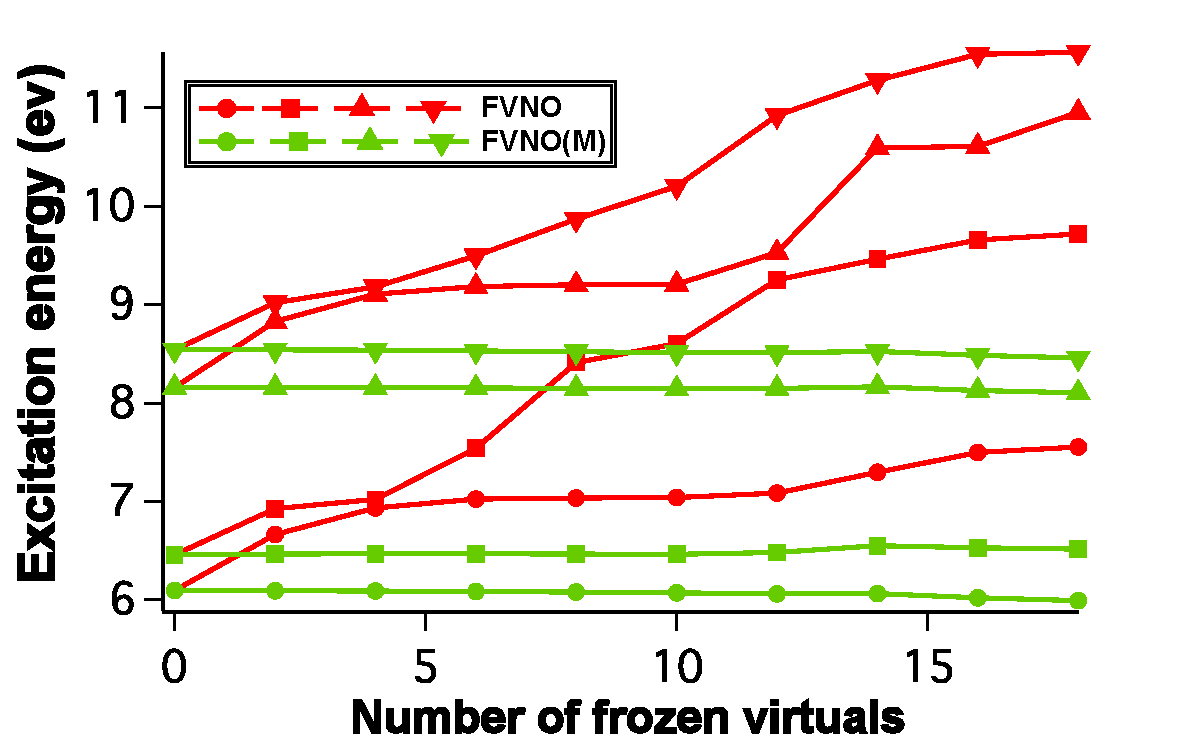
\includegraphics[width=.9\linewidth]{figures_fvno++/fvno(m)_h2o2_adz_ee.pdf}
%  \caption{}
%  \label{fig:sfig1}
%\end{subfigure}%
%\begin{subfigure}{.5\textwidth}
%  \centering
%  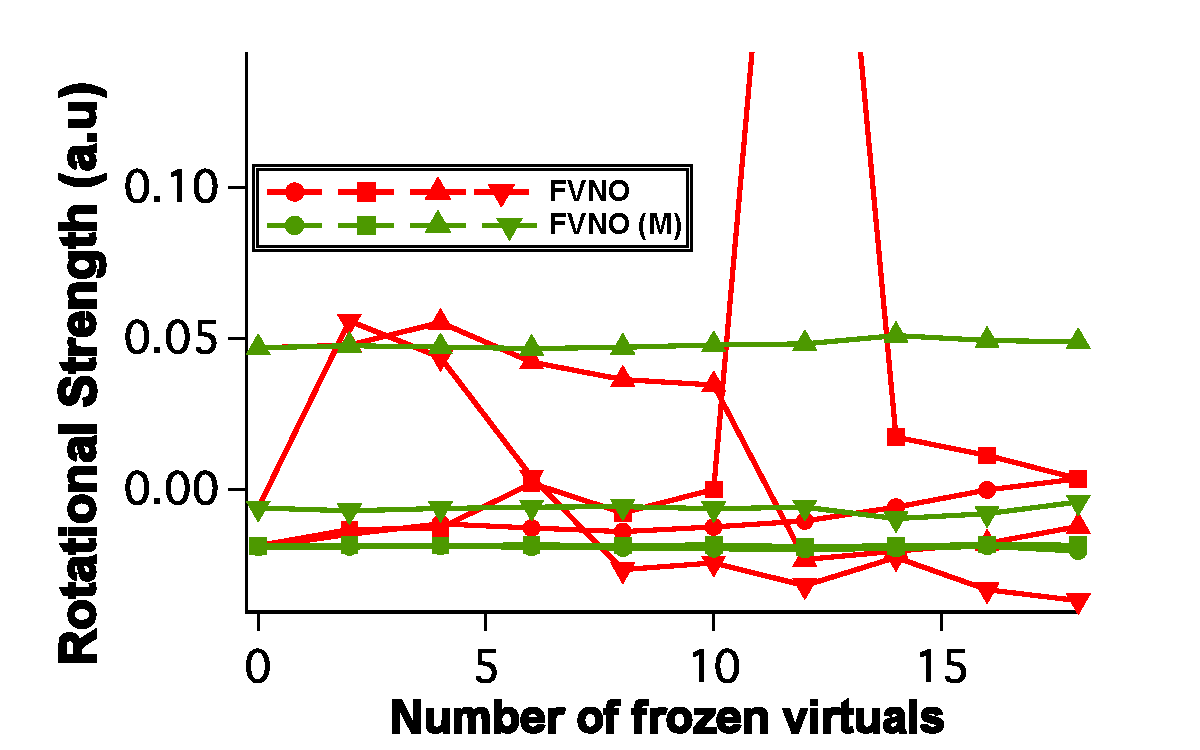
\includegraphics[width=.9\linewidth]{figures_fvno++/fvno(m)_h2o2_adz_rs.pdf}
%  \caption{}
%  \label{fig:sfig2}
%\end{subfigure}
%\caption{{\footnotesize EOM-CCSD/aDZ Oscillator (a) and Rotational (b) strengths of the lowest four excited states of H$_2$O$_2$ in both FVNO and FVNO(M) schemes as a function of the number of virtual orbitals removed.}}
%\label{fig:fvno(m)_h2o2_adz_ee_rs.pdf}
%\end{figure}
%%%%%%%%%%%%%%%%%%%%%%%%%%%%%%%%%%%%%%%%%%%%%%%%%%%%%%%%%%%%%%%%%%%%%%%%
\begin{figure}
\begin{subfigure}{.5\textwidth}
  \centering
  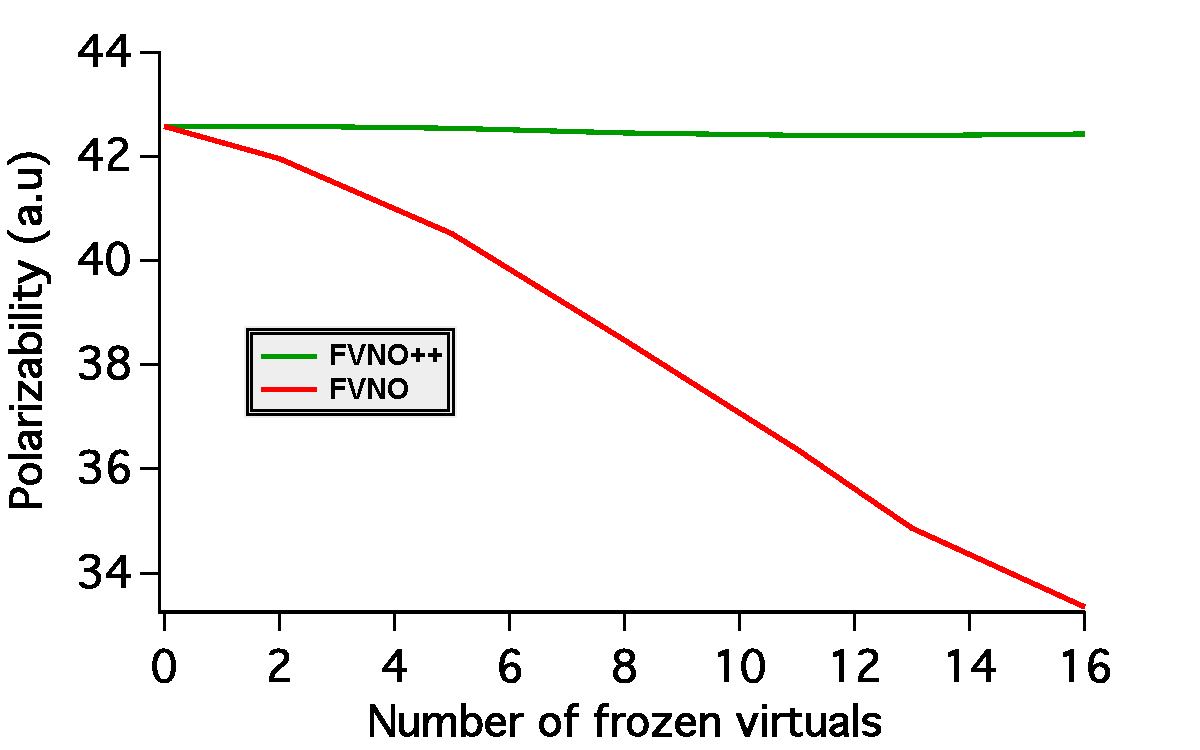
\includegraphics[width=.9\linewidth]{figures_fvno++/fvno++_h2o2_adz_polar.pdf}
  \caption{}
  \label{fig:sfig1}
\end{subfigure}%
\begin{subfigure}{.5\textwidth}
  \centering
  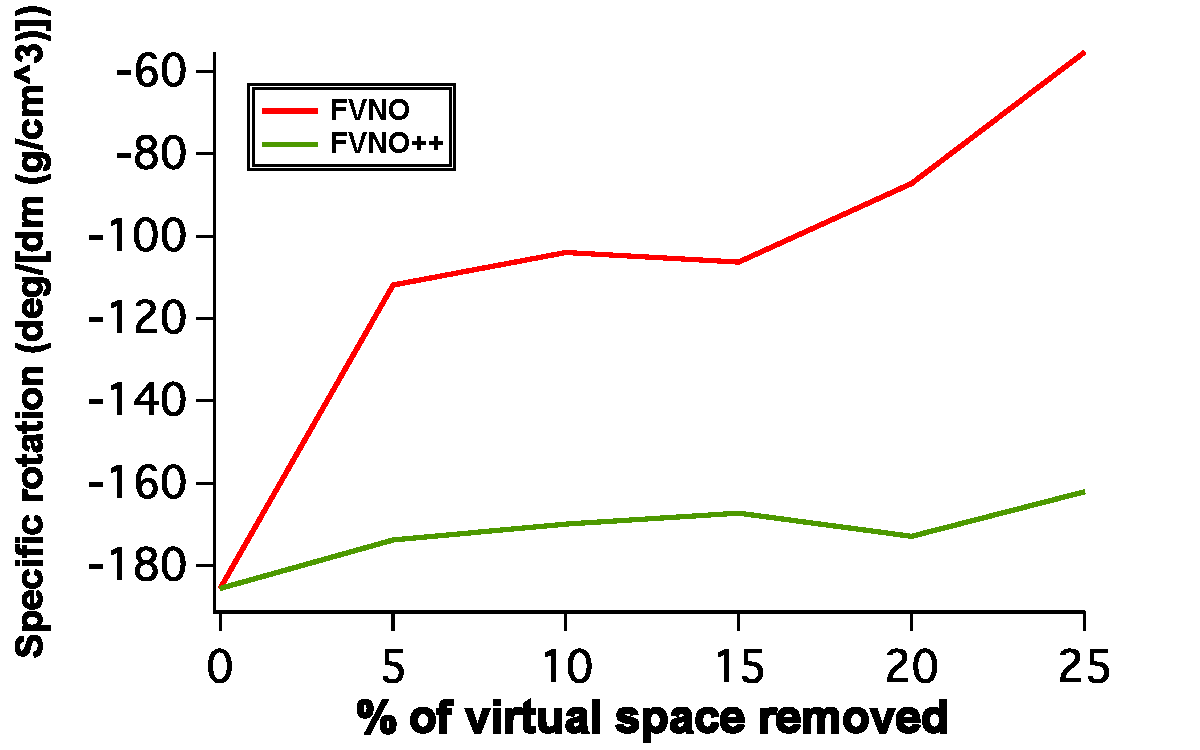
\includegraphics[width=.9\linewidth]{figures_fvno++/fvno++_h2o2_adz_optrot_lg.pdf}
  \caption{}
  \label{fig:sfig2}
\end{subfigure}
\caption{{\footnotesize CCSD/aDZ dynamic polarizabilities (a) and specific rotations (b) of H$_2$O$_2$ in both FVNO and FVNO++ schemes as a function of
number of virtual orbitals removed.}}
\label{fig:fvno++_h2o2_adz_polar_optrot_lg}
\end{figure}
%\begin{MyFigure}[h!]
%\centering
%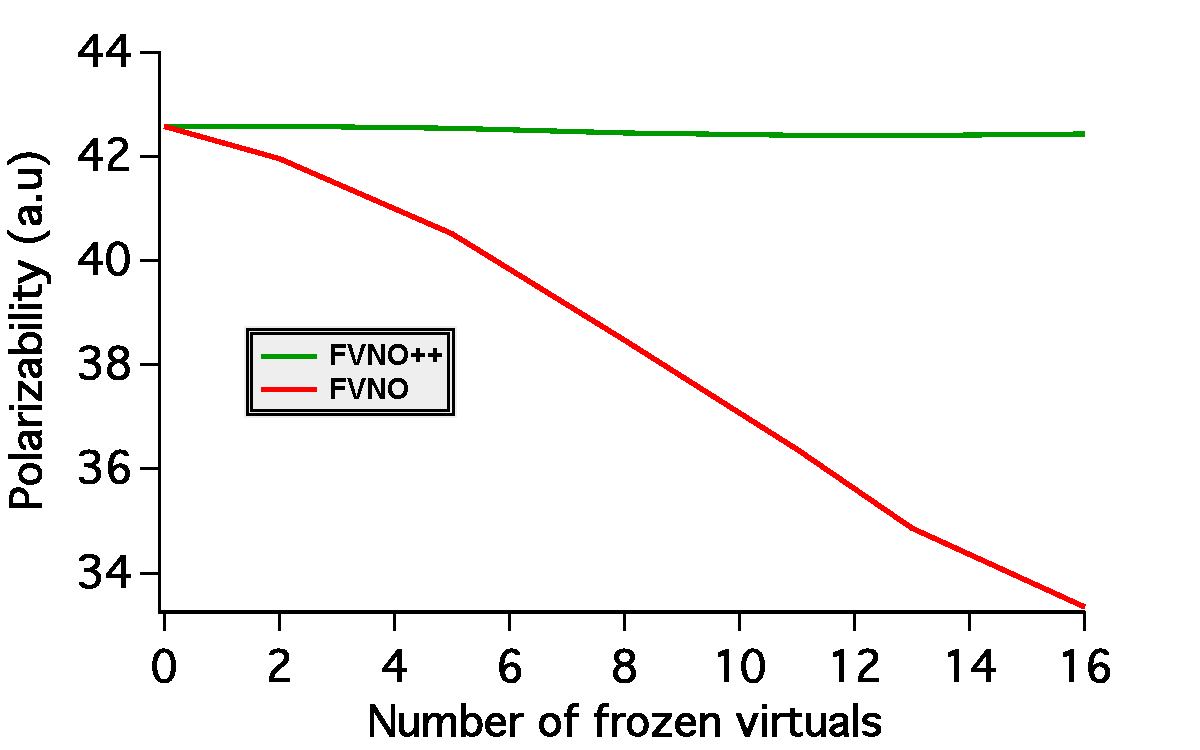
\includegraphics[width=0.5\linewidth]{figures_fvno++/fvno++_h2o2_adz_polar.pdf}
%\caption{{\footnotesize CCSD/aDZ polarizabilities of
%H$_2$O$_2$ in both FVNO and FVNO++ schemes as a function of
%number of virtual orbitals removed.}}
%\label{fig:fvno++_polar}
%\end{MyFigure}
compares the performances of both FVNO and FVNO++($\mu$) approaches
for calculating CCSD dynamic polarizabilities and specific rotations for the same system 
as above. The FVNO++ scheme indeed captures the contribution of VNOs to
the response of the wavefunction in the right manner. As a result, the removal of VNOs with low ONs
seem to have negligible effect on both polarizabilities and specific rotations.
%Fig.~\ref{fig:fvno++_optrot},
%\begin{MyFigure}[h!]
%\centering
%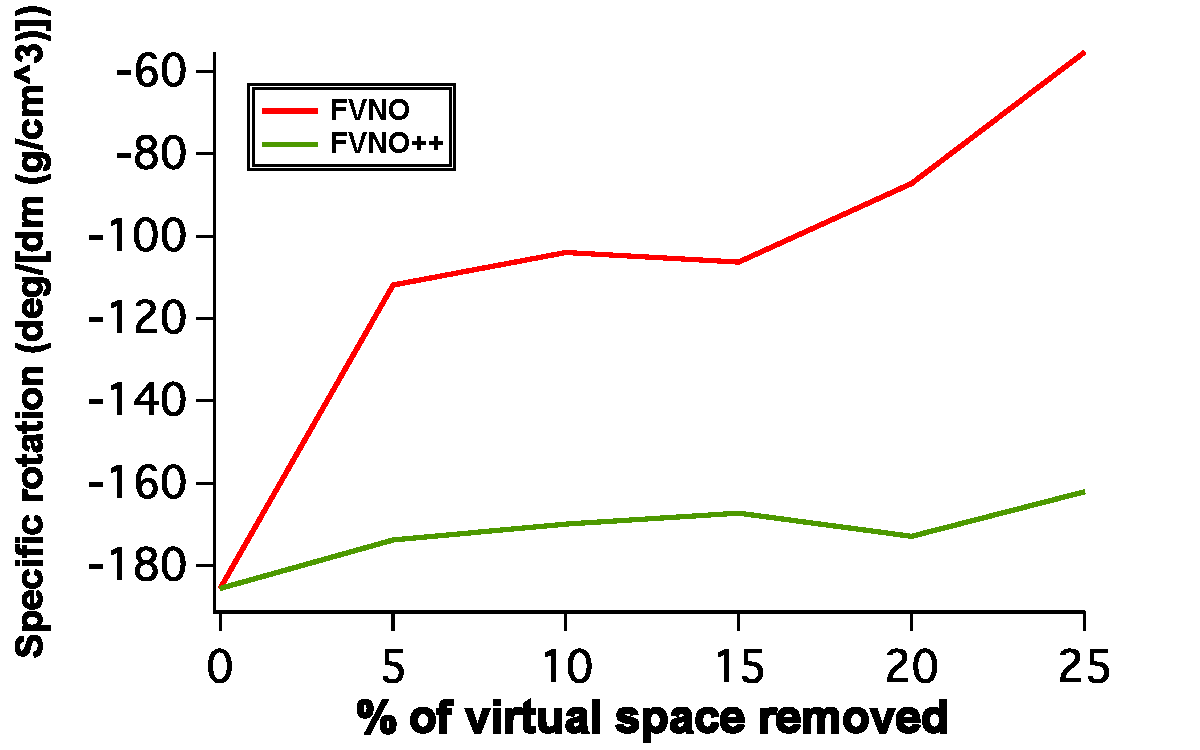
\includegraphics[width=0.5\linewidth]{figures_fvno++/fvno++_h2o2_adz_optrot_lg.pdf}
%\caption{{\footnotesize CCSD/aDZ/LG specific rotations of
%H$_2$O$_2$ in both FVNO and FVNO++ schemes as a function of
%number of virtual orbitals removed.}}
%\label{fig:fvno++_optrot}
%\end{MyFigure}
%which plots the errors in the LG specific rotations in both FVNO and FVNO++ schemes 
%also shows similar trends. 
Specific rotations can be seen to be more sensitive than polarizabilities with respect to 
truncation of orbitals in both the methods. However, the FVNO++ curve shows a systematic 
increase in error as more and more VNOs are removed while the errors in the FVNO procedure 
are at best erratic. 
%\begin{figure}[ht] \label{ fig7} 
%  \begin{minipage}[b]{0.5\linewidth}
%    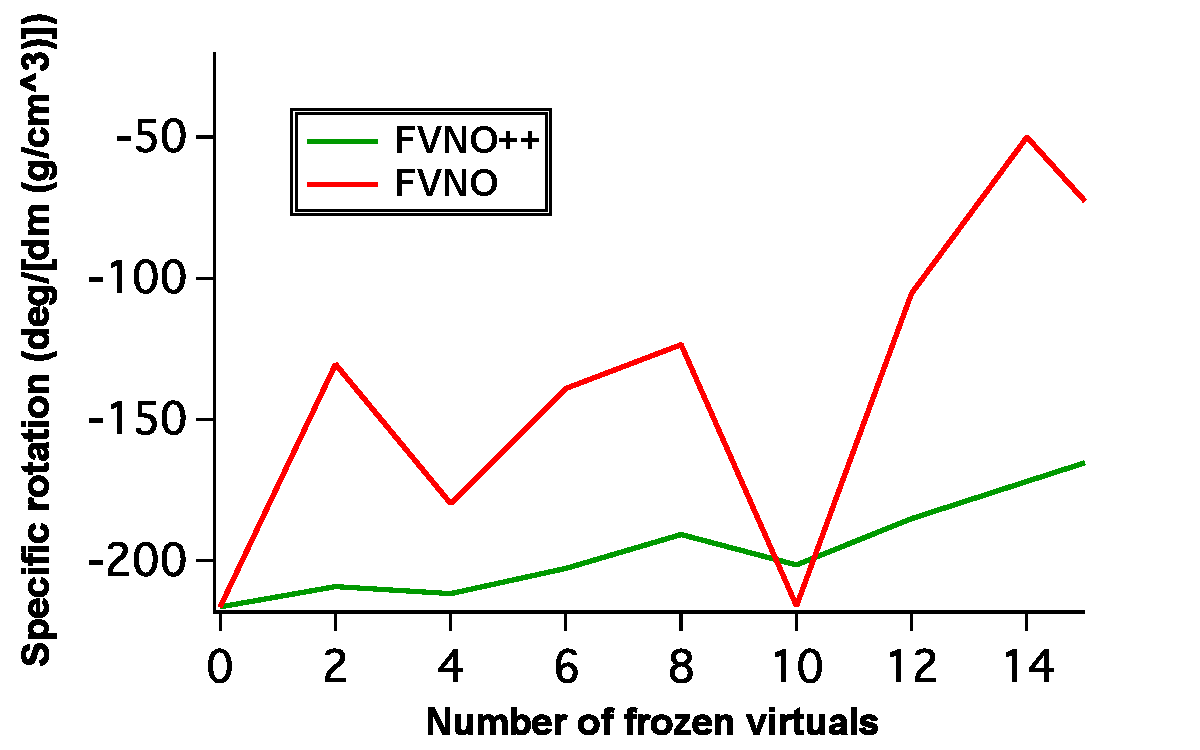
\includegraphics[width=.7\linewidth]{figures_fvno++/fvno++_h2o2_adz_optrot.pdf}
%    \caption{Initial condition} 
%  \end{minipage} 
%  \begin{minipage}[b]{0.5\linewidth}
%    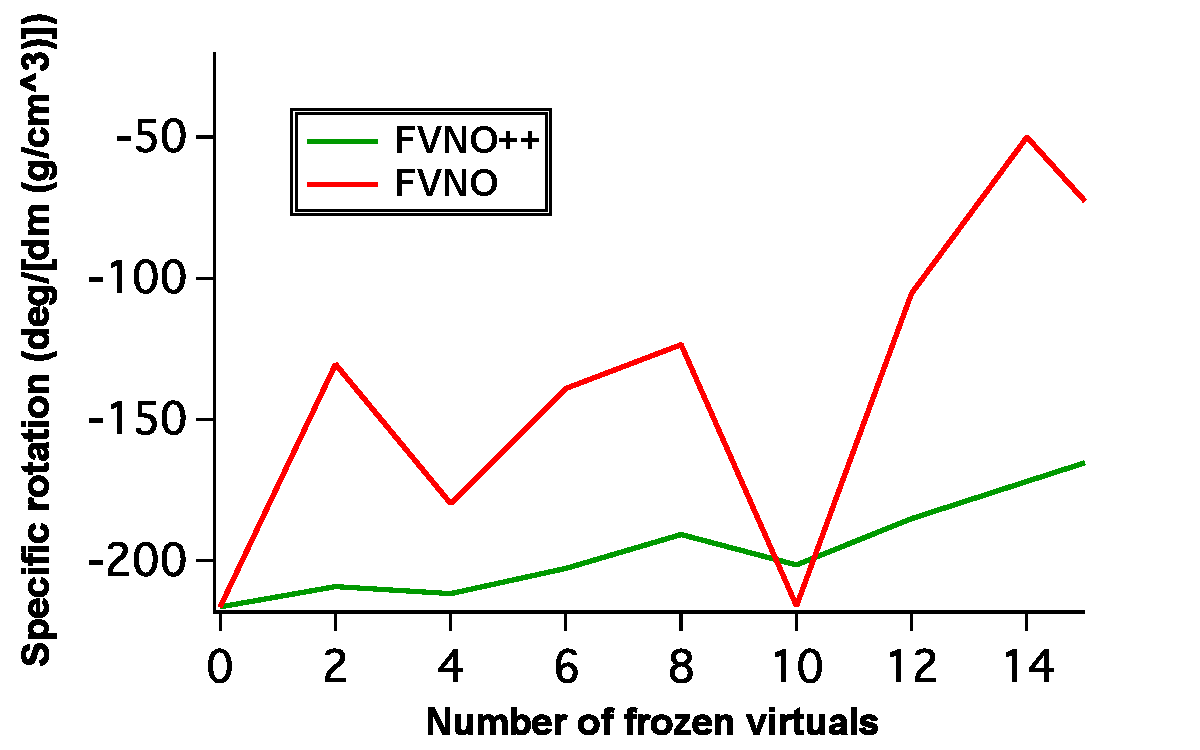
\includegraphics[width=.7\linewidth]{figures_fvno++/fvno++_h2o2_adz_optrot.pdf}
%    \caption{Rupture} 
%  \end{minipage} 
%  \begin{minipage}[b]{0.5\linewidth}
%    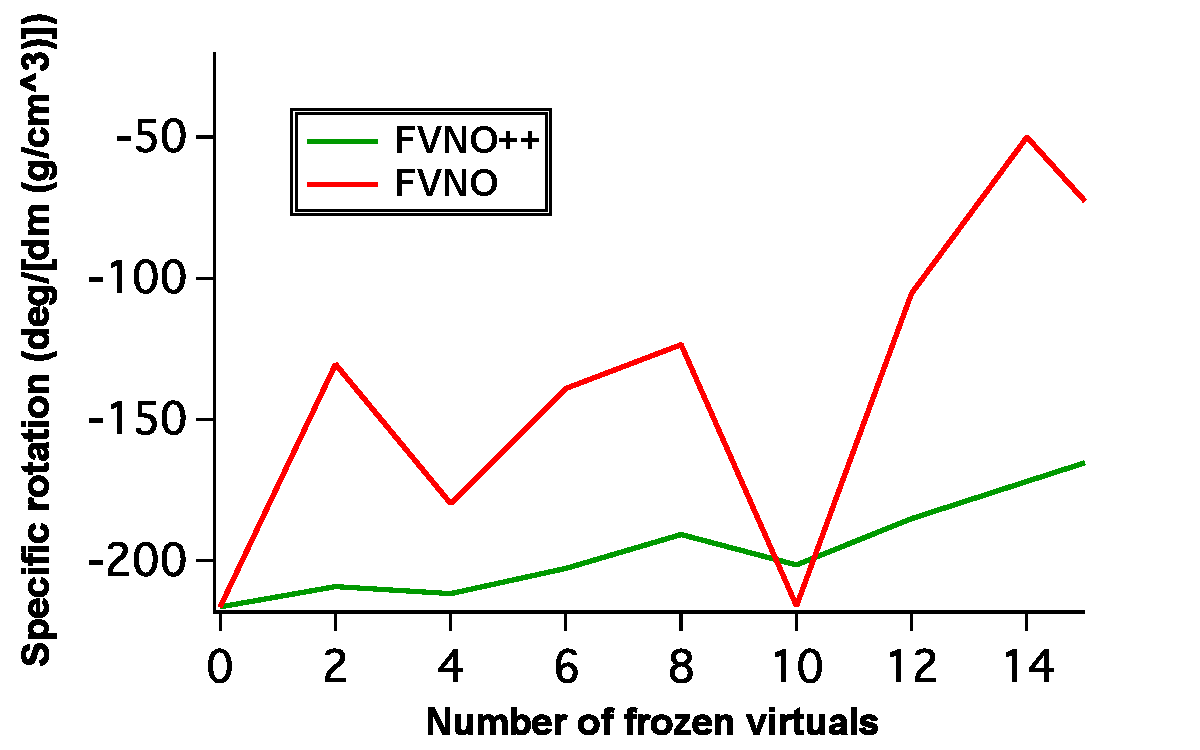
\includegraphics[width=.7\linewidth]{figures_fvno++/fvno++_h2o2_adz_optrot.pdf}
%    \caption{DFT, Initial condition} 
%  \end{minipage}
%  \hfill
%  \begin{minipage}[b]{0.5\linewidth}
%    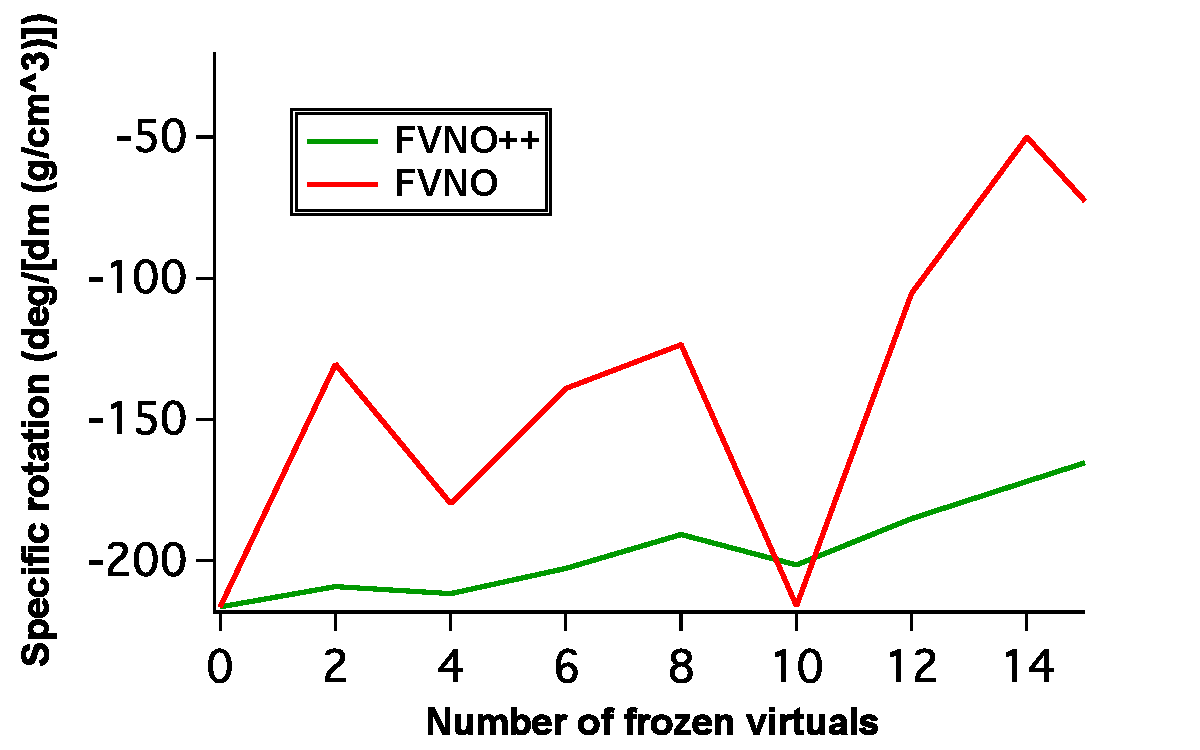
\includegraphics[width=.7\linewidth]{figures_fvno++/fvno++_h2o2_adz_optrot.pdf}
%    \caption{DFT, rupture} 
%  \end{minipage} 
%\end{figureA
Fig.~\ref{fig:fvno++_polar_h2_n} and Fig.~\ref{fig:fvno++_optrot_h2_n} extends the comparison of the two schemes 
to the linear (H$_2$)$_n$ helices.
\begin{figure}
\begin{subfigure}{.5\textwidth}
  \centering
  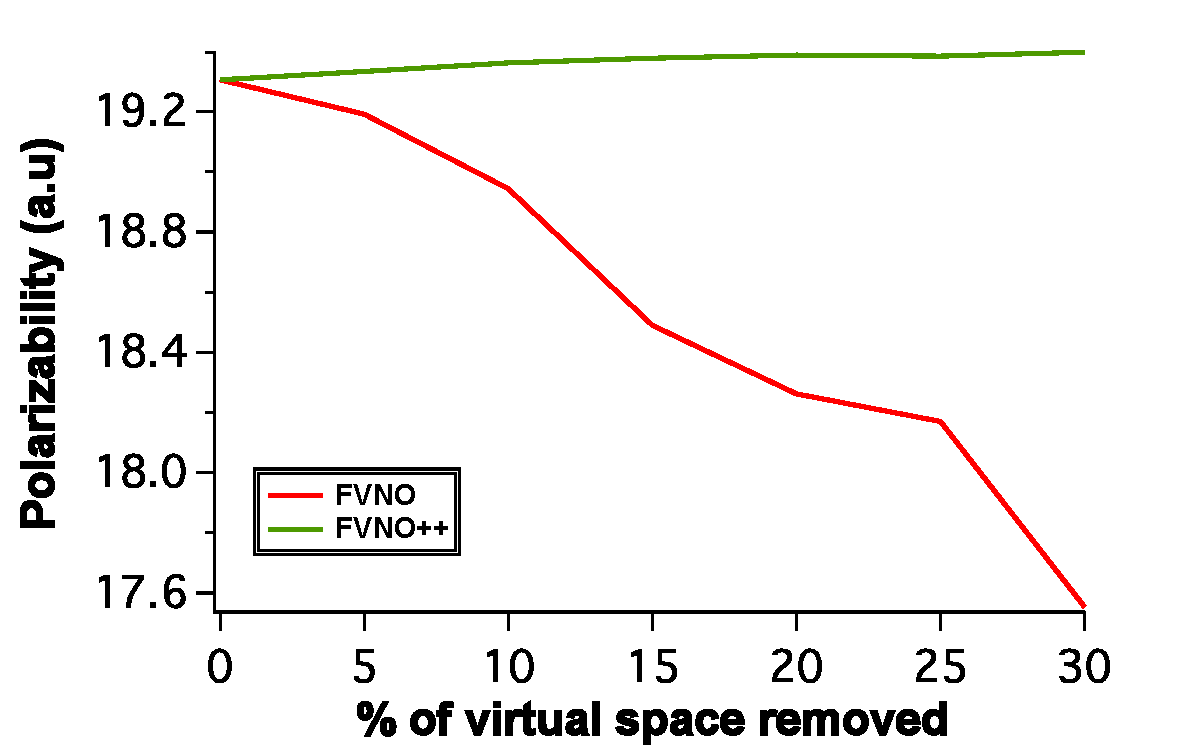
\includegraphics[width=.9\linewidth]{figures_fvno++/fvno++_h2_4_adz_polar.pdf}
  \caption{(H$_2$)$_4$}
  \label{fig:sfig1}
\end{subfigure}%
\begin{subfigure}{.5\textwidth}
  \centering
  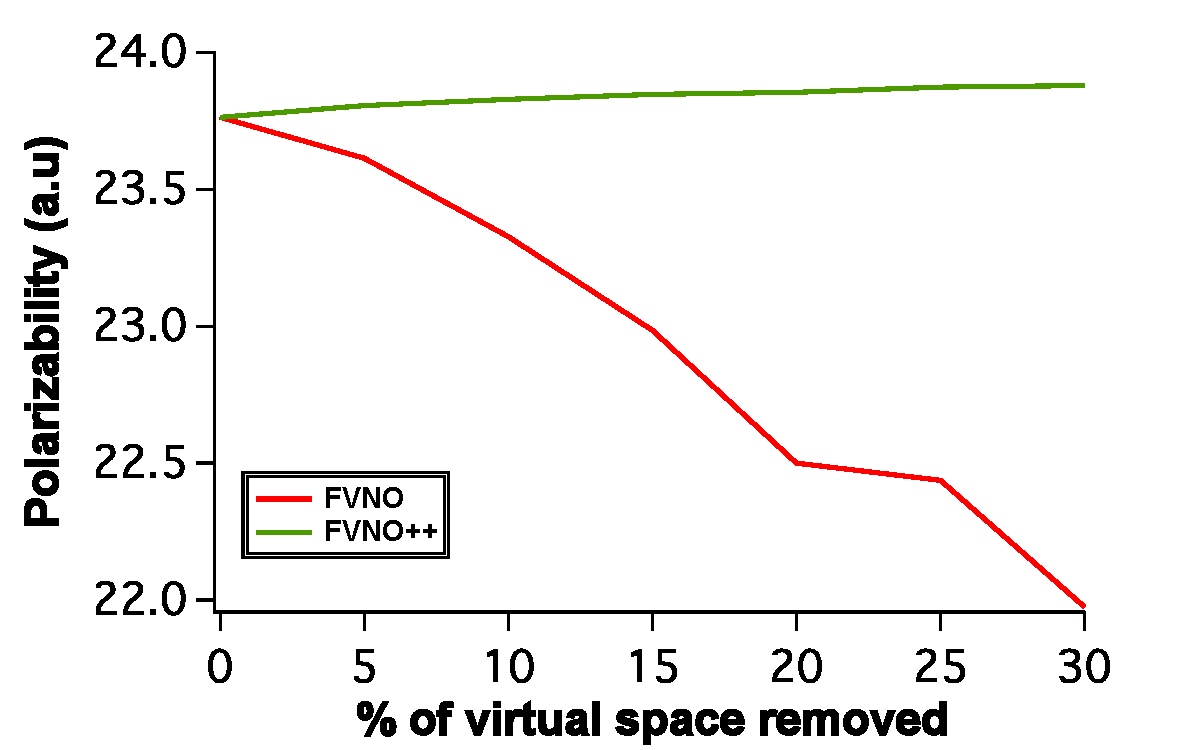
\includegraphics[width=.9\linewidth]{figures_fvno++/fvno++_h2_5_adz_polar.pdf}
  \caption{(H$_2$)$_5$}
  \label{fig:sfig2}
\end{subfigure}
\begin{subfigure}{.5\textwidth}
  \centering
  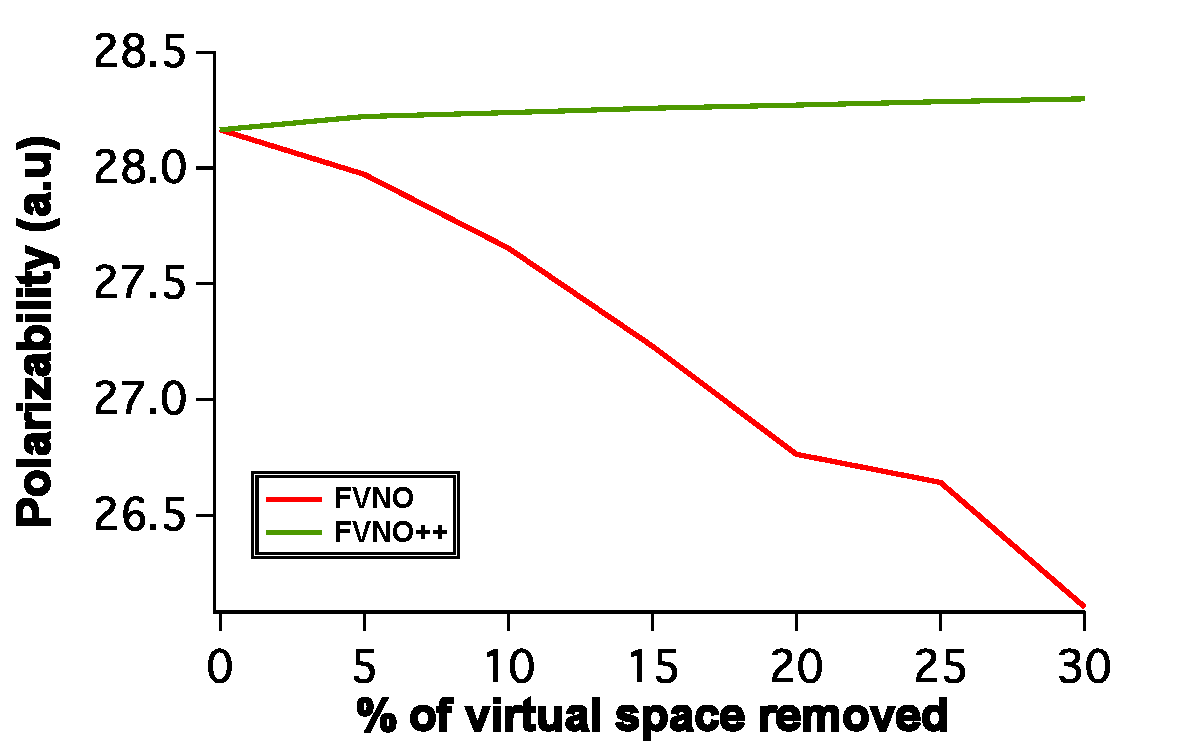
\includegraphics[width=.9\linewidth]{figures_fvno++/fvno++_h2_6_adz_polar.pdf}
  \caption{(H$_2$)$_6$}
  \label{fig:sfig2}
\end{subfigure}
\begin{subfigure}{.5\textwidth}
  \centering
  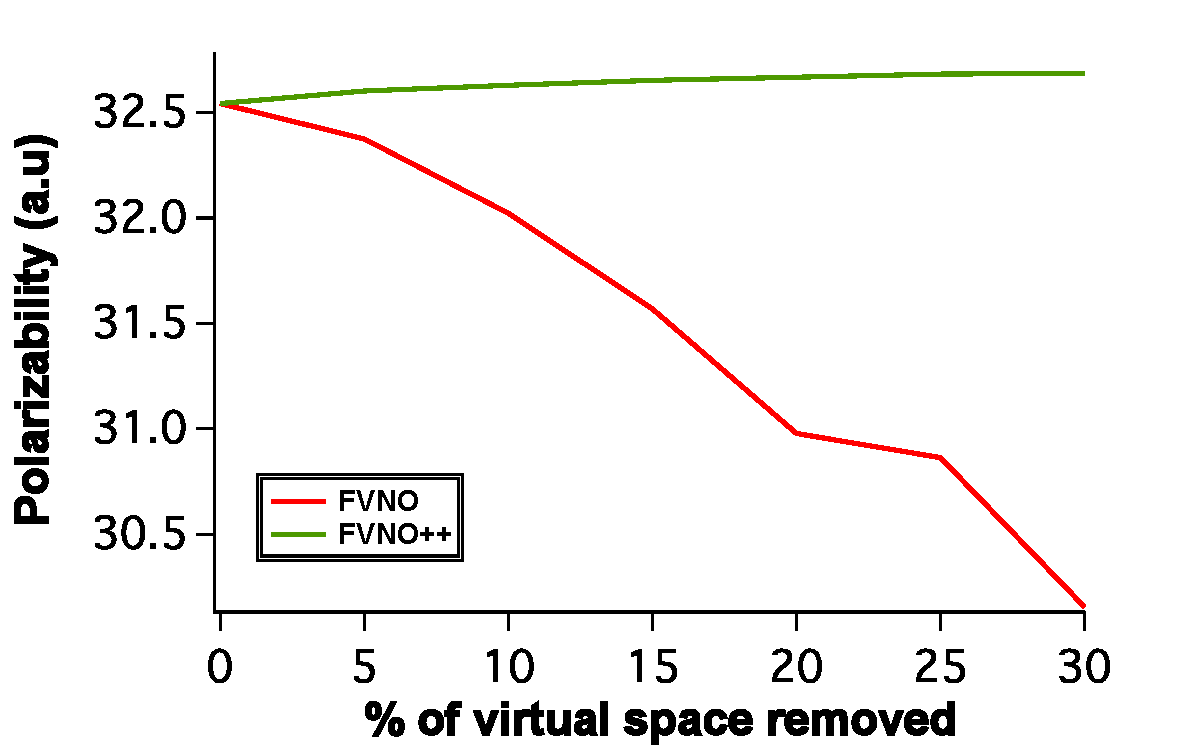
\includegraphics[width=.9\linewidth]{figures_fvno++/fvno++_h2_7_adz_polar.pdf}
  \caption{(H$_2$)$_7$}
  \label{fig:sfig2}
\end{subfigure}
\caption{{\footnotesize CCSD/aDZ polarizabilities of
(H$_2$)$_n$ helices, $ n = 4-7$ in both FVNO and FVNO++ schemes as a function of
percentage of virtual space removed.}}
\label{fig:fvno++_polar_h2_n}
\end{figure}
%%%%%%%%%%%%%%%%%%%%%%%%%%%%%%%%%%%%%%%%%%%%%%%%%%%%%%%%%%%%%%%%%%%%%%%%%%%
\begin{figure}
\begin{subfigure}{.5\textwidth}
  \centering
  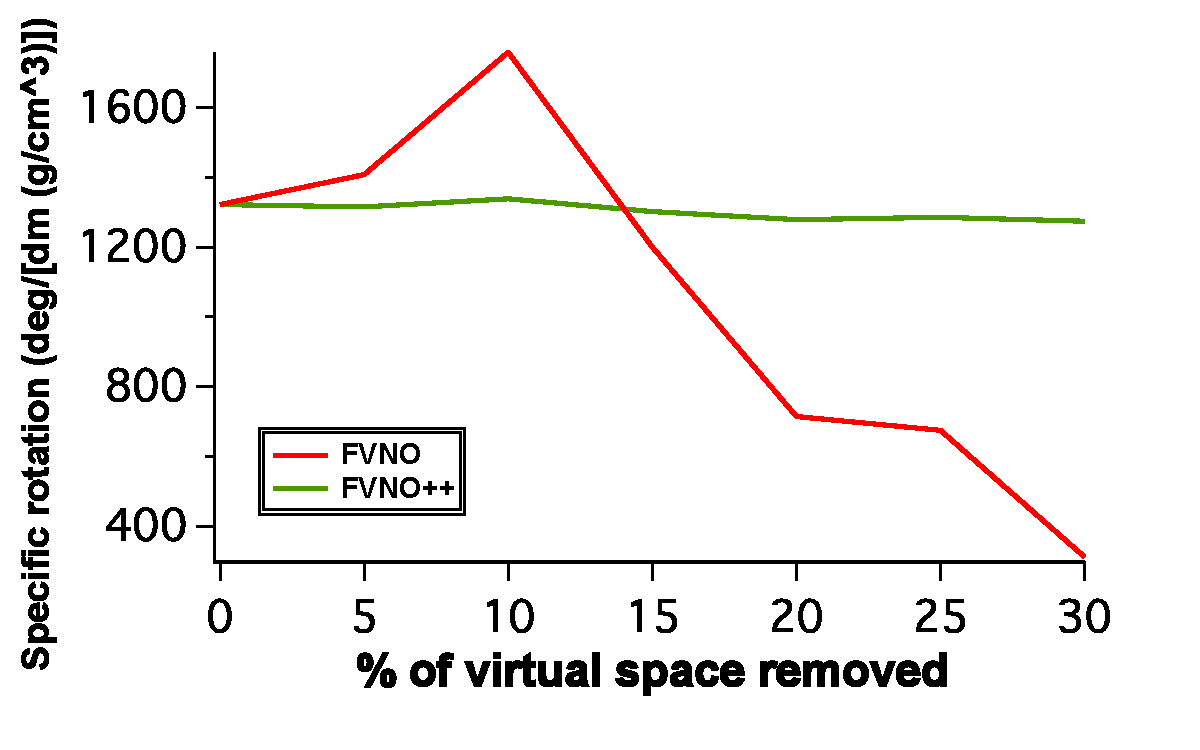
\includegraphics[width=.9\linewidth]{figures_fvno++/fvno++_h2_4_adz_optrot_lg.pdf}
  \caption{(H$_2$)$_4$}
  \label{fig:sfig1}
\end{subfigure}%
\begin{subfigure}{.5\textwidth}
  \centering
  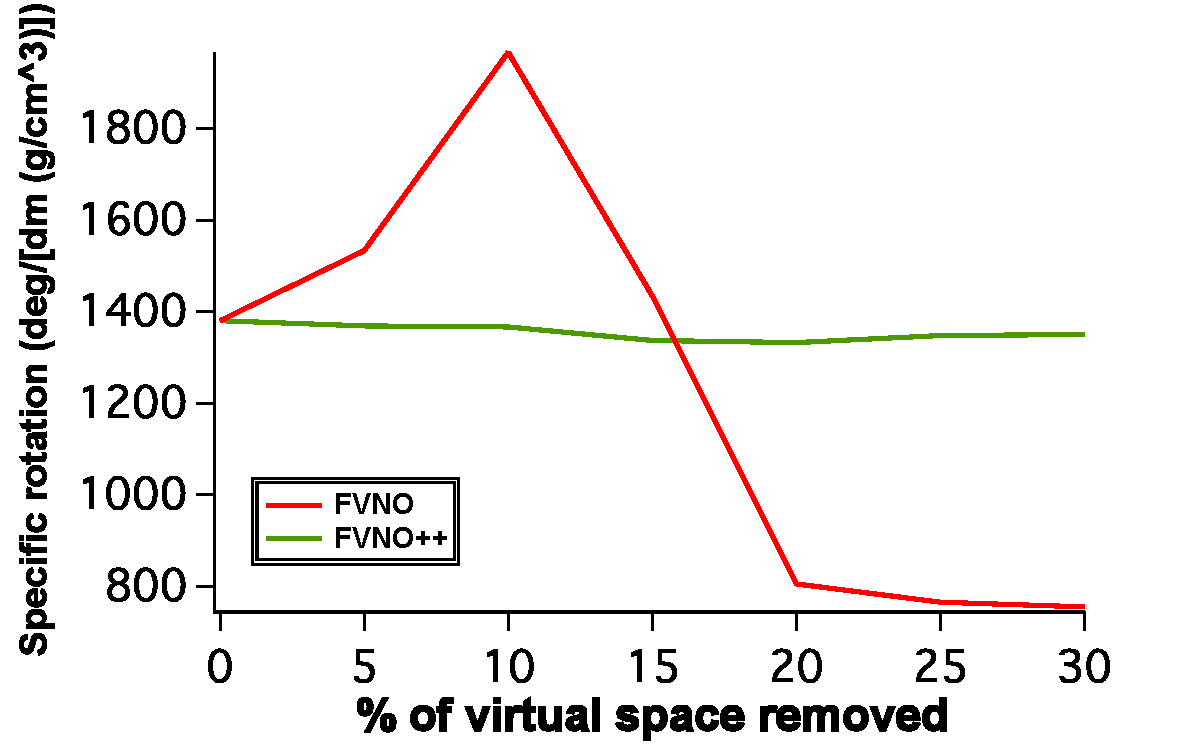
\includegraphics[width=.9\linewidth]{figures_fvno++/fvno++_h2_5_adz_optrot_lg.pdf}
  \caption{(H$_2$)$_5$}
  \label{fig:sfig2}
\end{subfigure}
\begin{subfigure}{.5\textwidth}
  \centering
  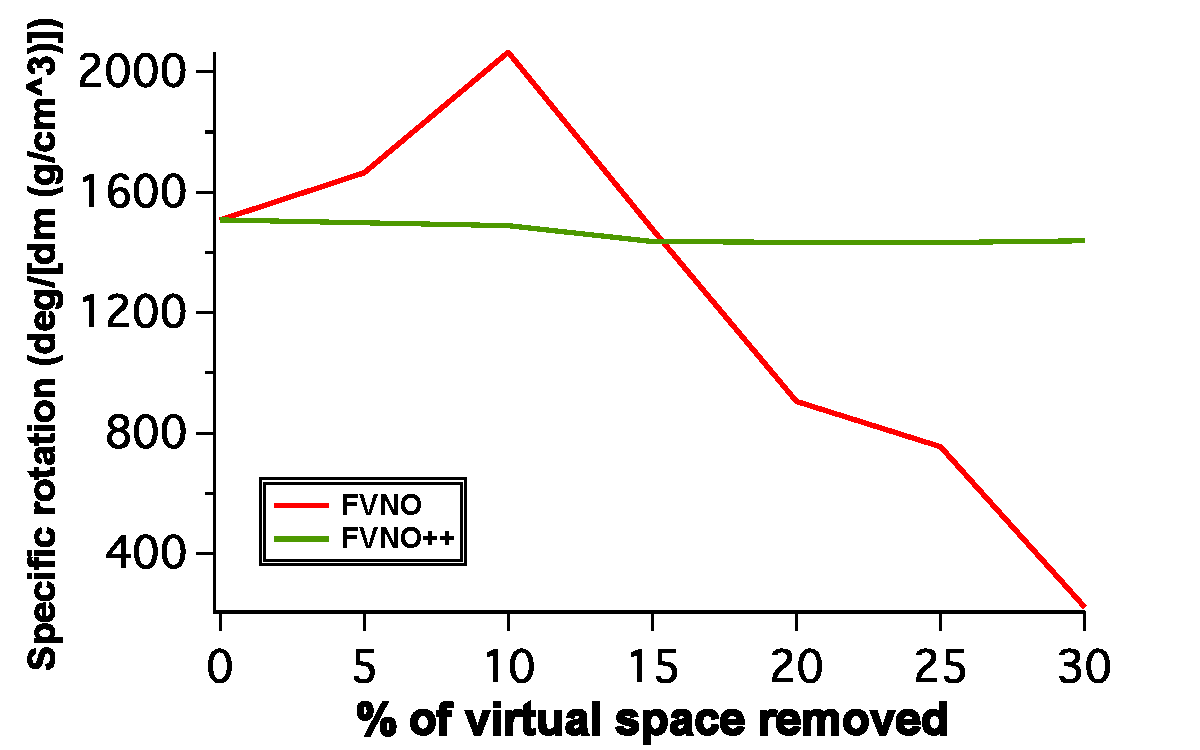
\includegraphics[width=.9\linewidth]{figures_fvno++/fvno++_h2_6_adz_optrot_lg.pdf}
  \caption{(H$_2$)$_6$}
  \label{fig:sfig2}
\end{subfigure}
\begin{subfigure}{.5\textwidth}
  \centering
  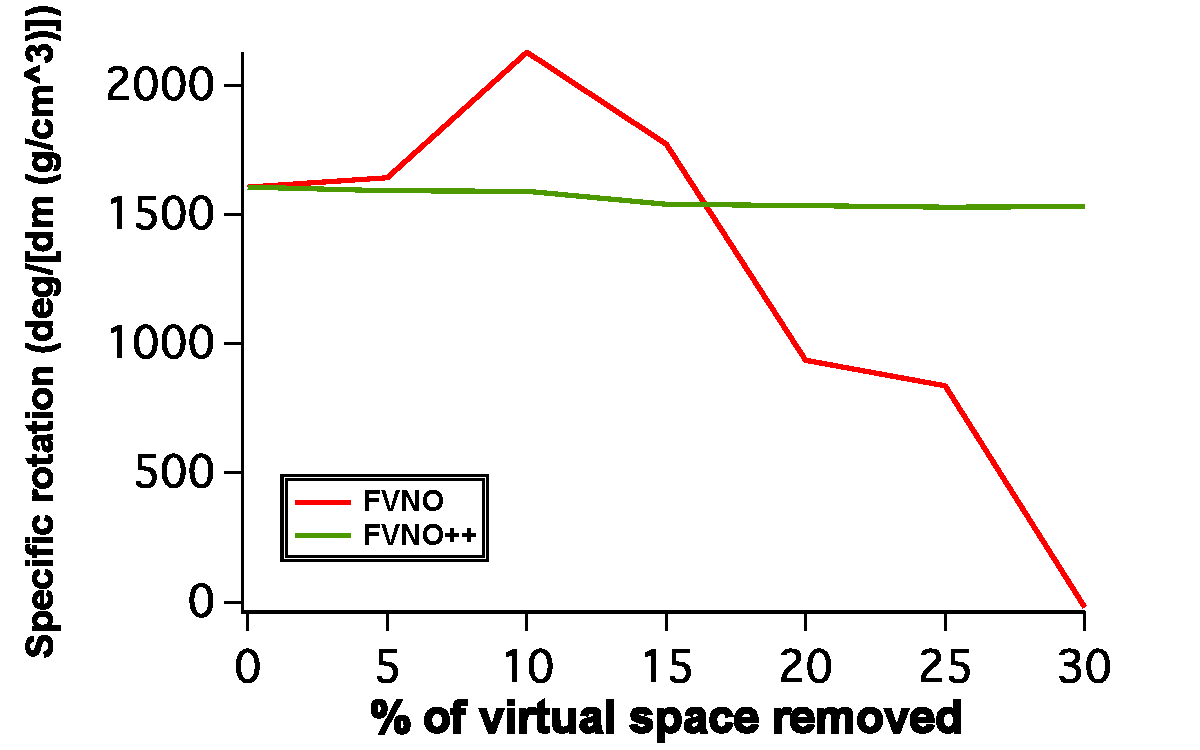
\includegraphics[width=.9\linewidth]{figures_fvno++/fvno++_h2_7_adz_optrot_lg.pdf}
  \caption{(H$_2$)$_7$}
  \label{fig:sfig2}
\end{subfigure}
\caption{{\footnotesize CCSD/aDZ  specific rotations of
(H$_2$)$_n$ helices, $ n = 4-7$ in both FVNO and FVNO++ schemes as a function of
percentage of virtual space removed.}}
\label{fig:fvno++_optrot_h2_n}
\end{figure}
As expected , the errors in the FVNO++ scheme for both polarizabilities and specific rotations are
very small even after the removal of as much as 30\% of the virtual space for all the four helices.
For the (H$_2$)$_7$ system, the errors in the polarizability in the FVNO and FVNO++ methods are 
approximately 7\% and 0.4\% respectively after truncation 30\% of VNOs. For the same system and truncation
percentage, the FVNO method gives opposite signs of specific rotations while the FVNO++ approach 
yields errors within 5\%. We also investigated if the truncation errors associated with the 
FVNO++ approach can be minimized by optimizing the guess densities. In this regard, we carry out 
one iteration of the CC2 response equations with MP2 amplitudes to obtain the perturbed amplitudes
to build the guess density. Fig.~\ref{fig:fvno++_polar_opt_h2_n} plots the polarizabilities 
obtained using this optimized density (FVNO++(1)) and compares them with the earlier approach (FVNO++(0)).
It can be easily seen that the VNOs obtained from FVNO++(1) method are significantly more 
compact in the truncation range of up to 20\%. However, the errors start increasing steeply thereafter
and become comparable with that of the FVNO++(0) approach indicating that the aDZ basis set for these small 
systems is fairly compact. 
\begin{figure}
\begin{subfigure}{.5\textwidth}
  \centering
  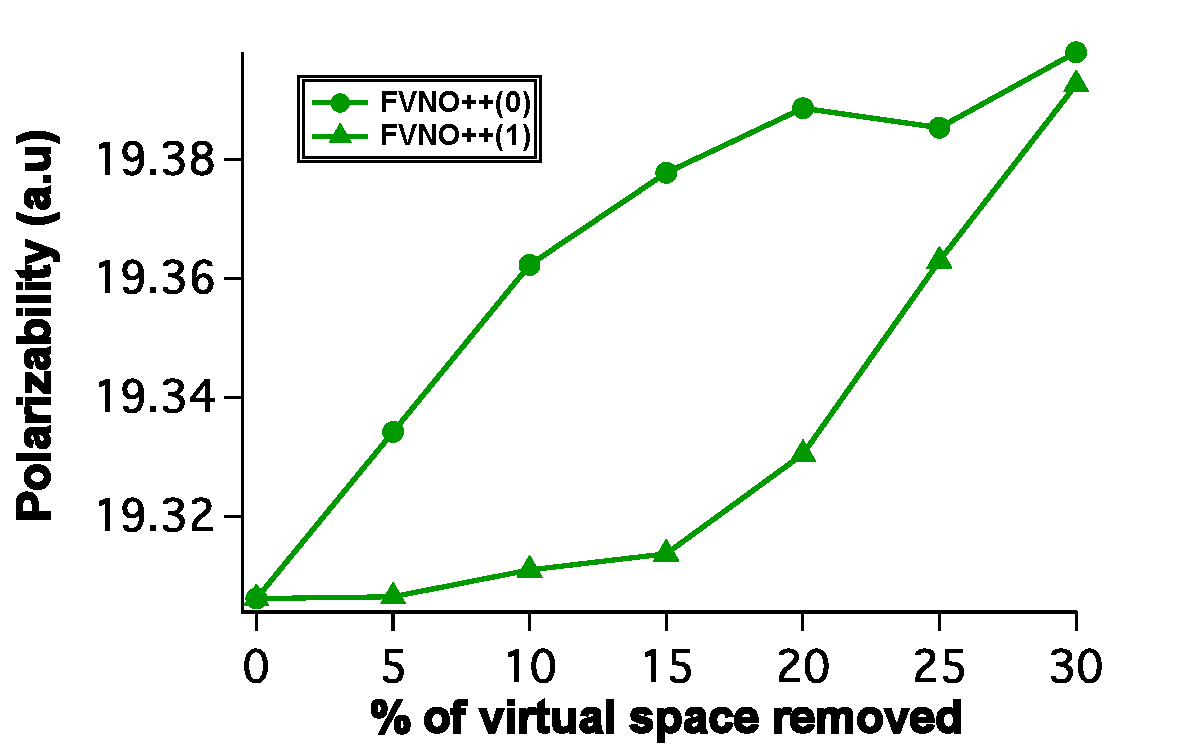
\includegraphics[width=.9\linewidth]{figures_fvno++/fvno++_cc2_1_h2_4_adz_polar.pdf}
  \caption{(H$_2$)$_4$}
  \label{fig:sfig1}
\end{subfigure}%
\begin{subfigure}{.5\textwidth}
  \centering
  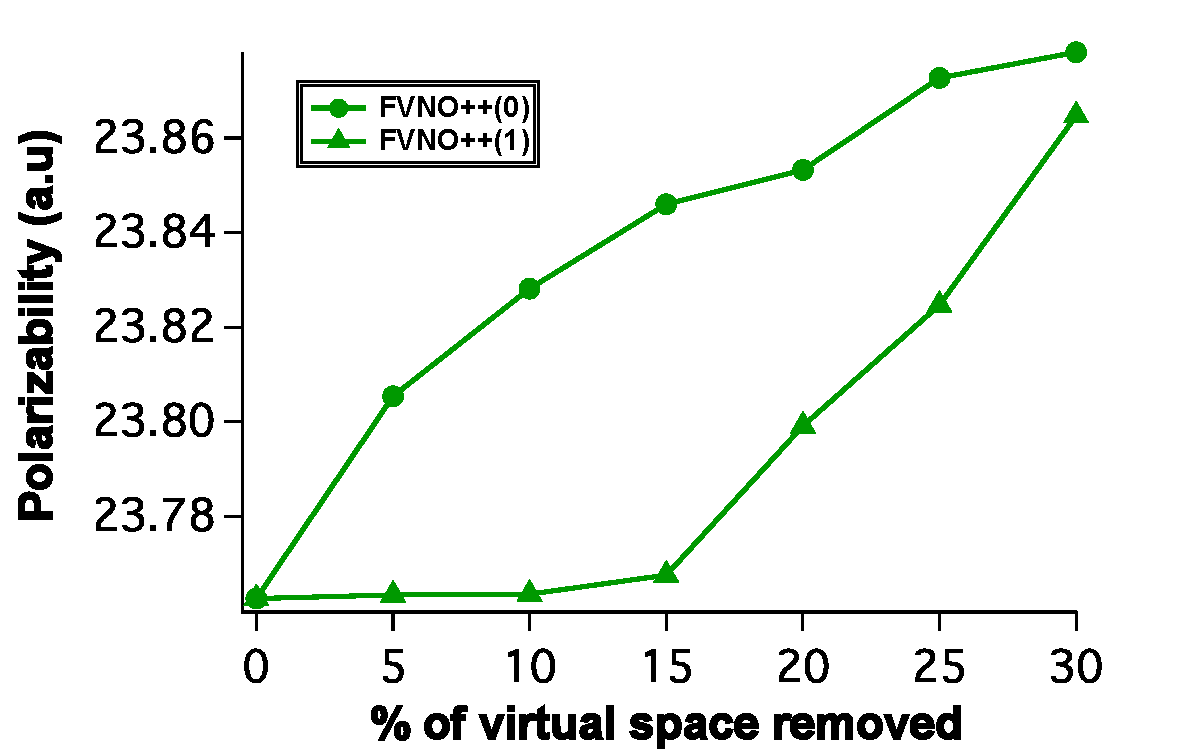
\includegraphics[width=.9\linewidth]{figures_fvno++/fvno++_cc2_1_h2_5_adz_polar.pdf}
  \caption{(H$_2$)$_5$}
  \label{fig:sfig2}
\end{subfigure}
\begin{subfigure}{.5\textwidth}
  \centering
  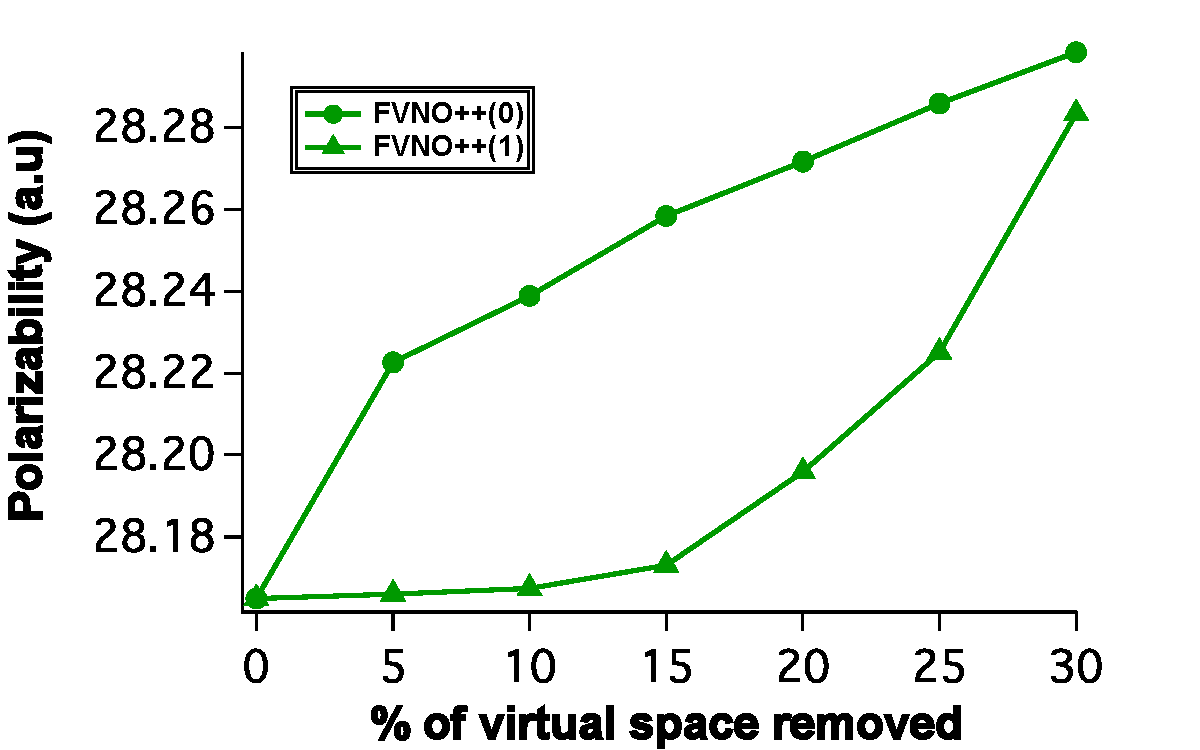
\includegraphics[width=.9\linewidth]{figures_fvno++/fvno++_cc2_1_h2_6_adz_polar.pdf}
  \caption{(H$_2$)$_6$}
  \label{fig:sfig2}
\end{subfigure}
\begin{subfigure}{.5\textwidth}
  \centering
  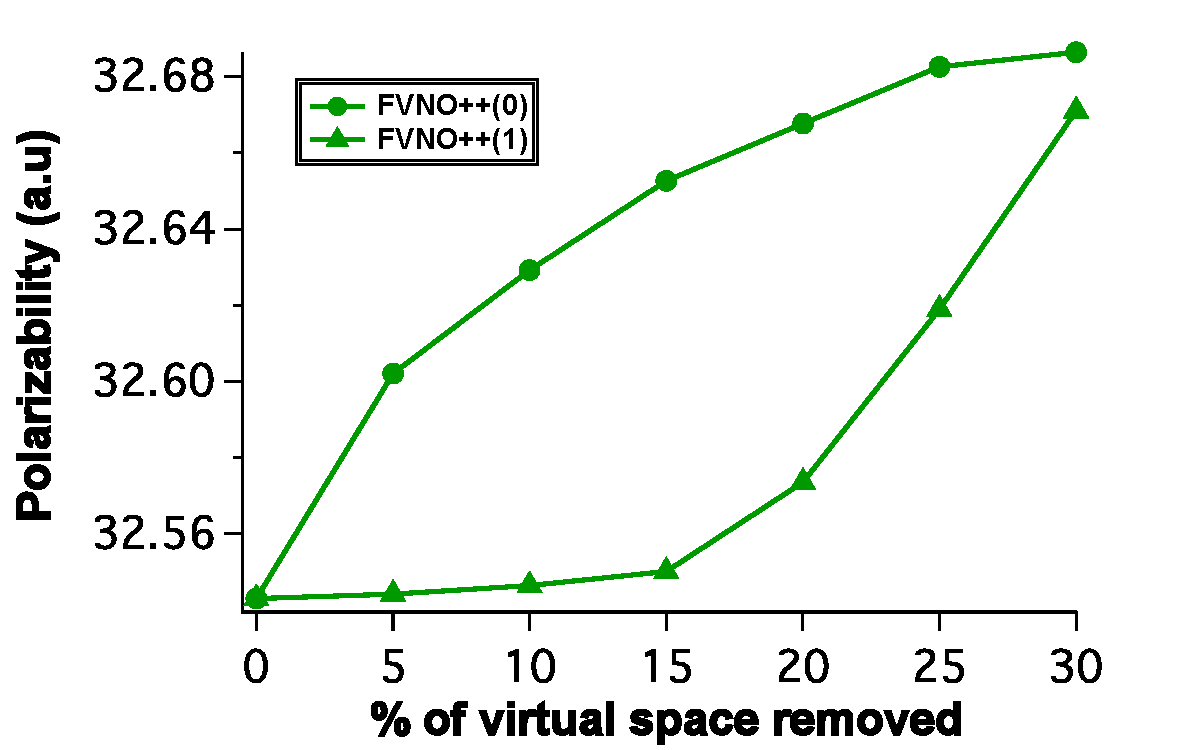
\includegraphics[width=.9\linewidth]{figures_fvno++/fvno++_cc2_1_h2_7_adz_polar.pdf}
  \caption{(H$_2$)$_7$}
  \label{fig:sfig2}
\end{subfigure}
\caption{{\footnotesize CCSD/aDZ polarizabilities of
(H$_2$)$_n$ helices, $ n = 4-7$ in both FVNO++(0) and FVNO++(1) schemes as a function of
percentage of virtual space removed.}}
\label{fig:fvno++_polar_opt_h2_n}
\end{figure}
%%%%%%%%%%%%%%%%%%%%%%%%%%%%%%%%%%%%%%%%%%%%%%%%%%%%%%%%%%%%%%%%%%%%%%%%%%%
For specific rotations, (fig.~\ref{fig:fvno++_optrot_opt_h2_n}) the results obtained 
using both the schemes are comparable up to a truncation of 10\% after which the errors in the FVNO++(0) 
method start rising sharply. For the (H$_2$)$_7$ molecule, the FVNO++(1) approach gave a maximum error of only 3\% (earlier 5\%) 
for the plotted truncation range.
\begin{figure}
\begin{subfigure}{.5\textwidth}
  \centering
  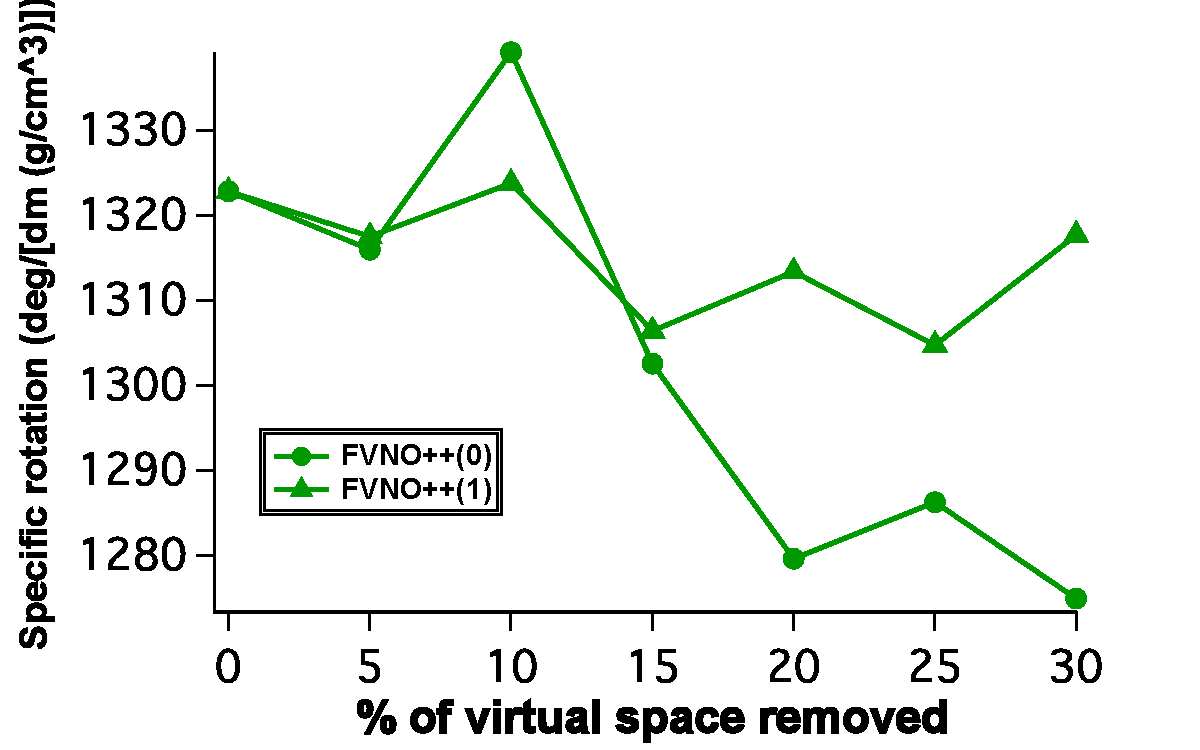
\includegraphics[width=.9\linewidth]{figures_fvno++/fvno++_cc2_1_h2_4_adz_optrot_lg.pdf}
  \caption{(H$_2$)$_4$}
  \label{fig:sfig1}
\end{subfigure}%
\begin{subfigure}{.5\textwidth}
  \centering
  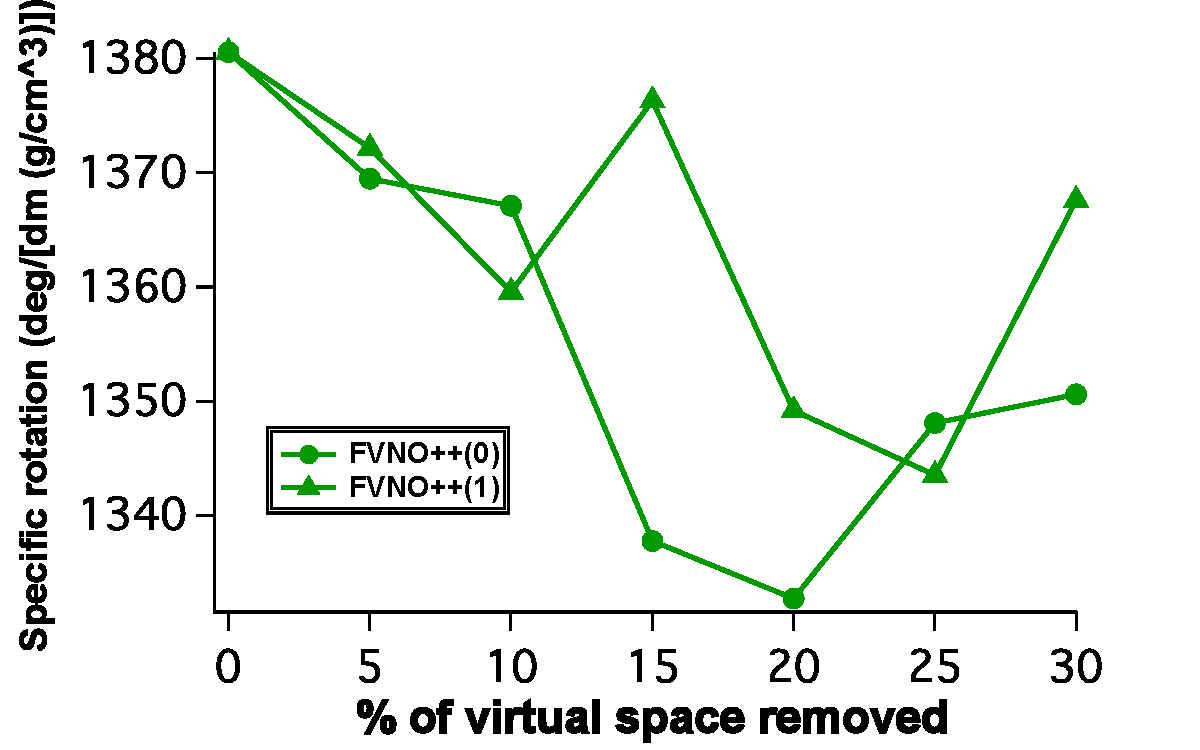
\includegraphics[width=.9\linewidth]{figures_fvno++/fvno++_cc2_1_h2_5_adz_optrot_lg.pdf}
  \caption{(H$_2$)$_5$}
  \label{fig:sfig2}
\end{subfigure}
\begin{subfigure}{.5\textwidth}
  \centering
  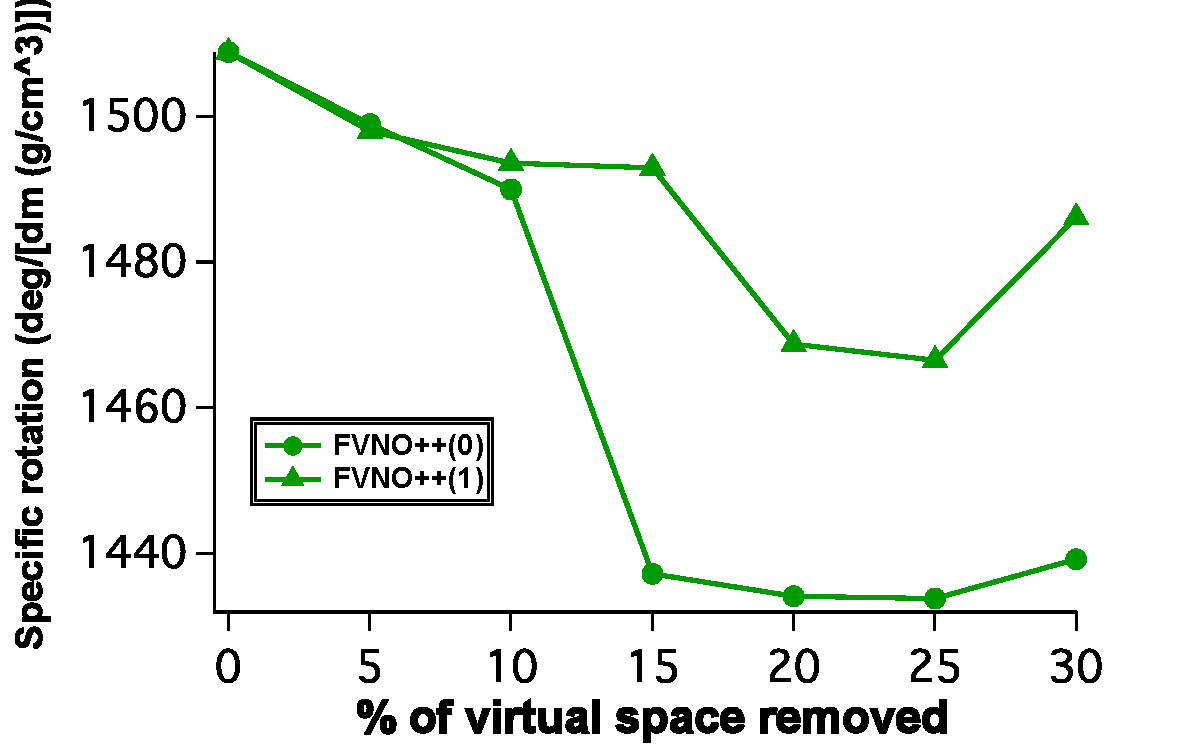
\includegraphics[width=.9\linewidth]{figures_fvno++/fvno++_cc2_1_h2_6_adz_optrot_lg.pdf}
  \caption{(H$_2$)$_6$}
  \label{fig:sfig2}
\end{subfigure}
\begin{subfigure}{.5\textwidth}
  \centering
  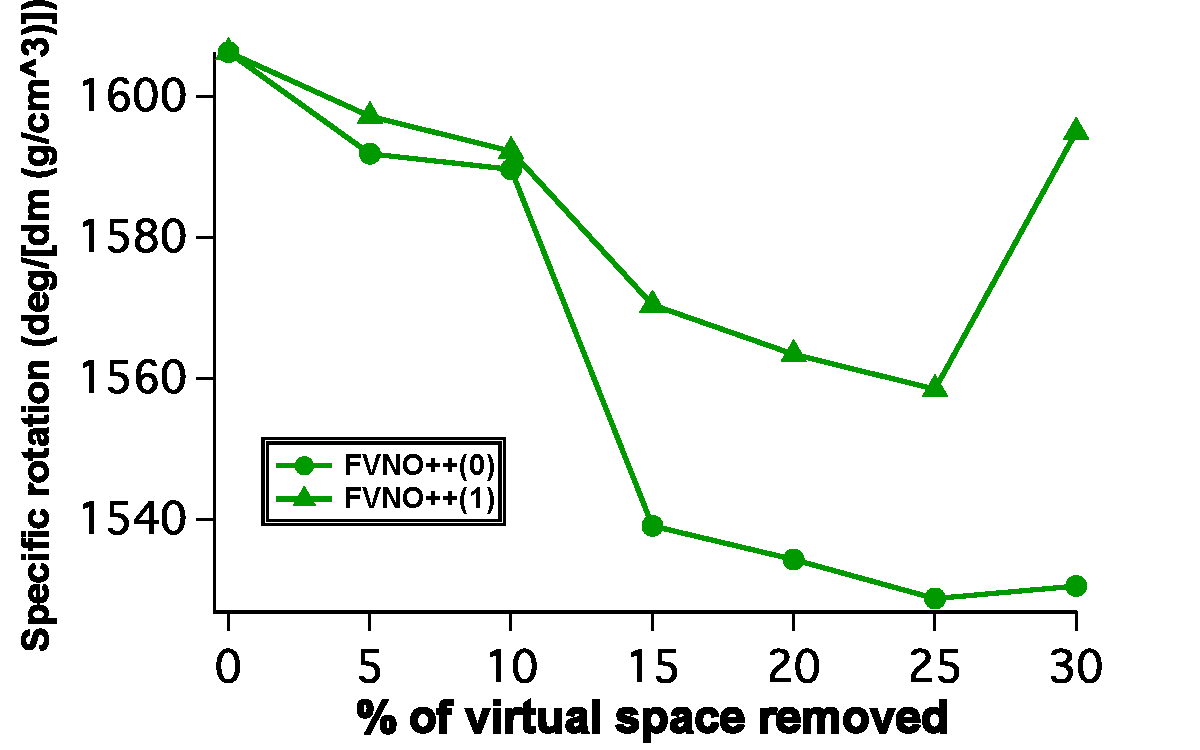
\includegraphics[width=.9\linewidth]{figures_fvno++/fvno++_cc2_1_h2_7_adz_optrot_lg.pdf}
  \caption{(H$_2$)$_7$}
  \label{fig:sfig2}
\end{subfigure}
\caption{{\footnotesize CCSD/aDZ specific rotations of
(H$_2$)$_n$ helices, $ n = 4-7$ in both FVNO++(0) and FVNO++(1) schemes as a function of
percentage of virtual space removed.}}
\label{fig:fvno++_optrot_opt_h2_n}
\end{figure}
\\
As mentioned before, we also tested the performance of two new approaches, FVNO++ ($\mu * L$)
and FVNO++ ($\mu,L$) for specific rotations for the (H$_2$)$_7$ molecule, see fig.~\ref{fig:fvno++_optrot_opt_h2_n}.
\begin{MyFigure}[h!]
\centering
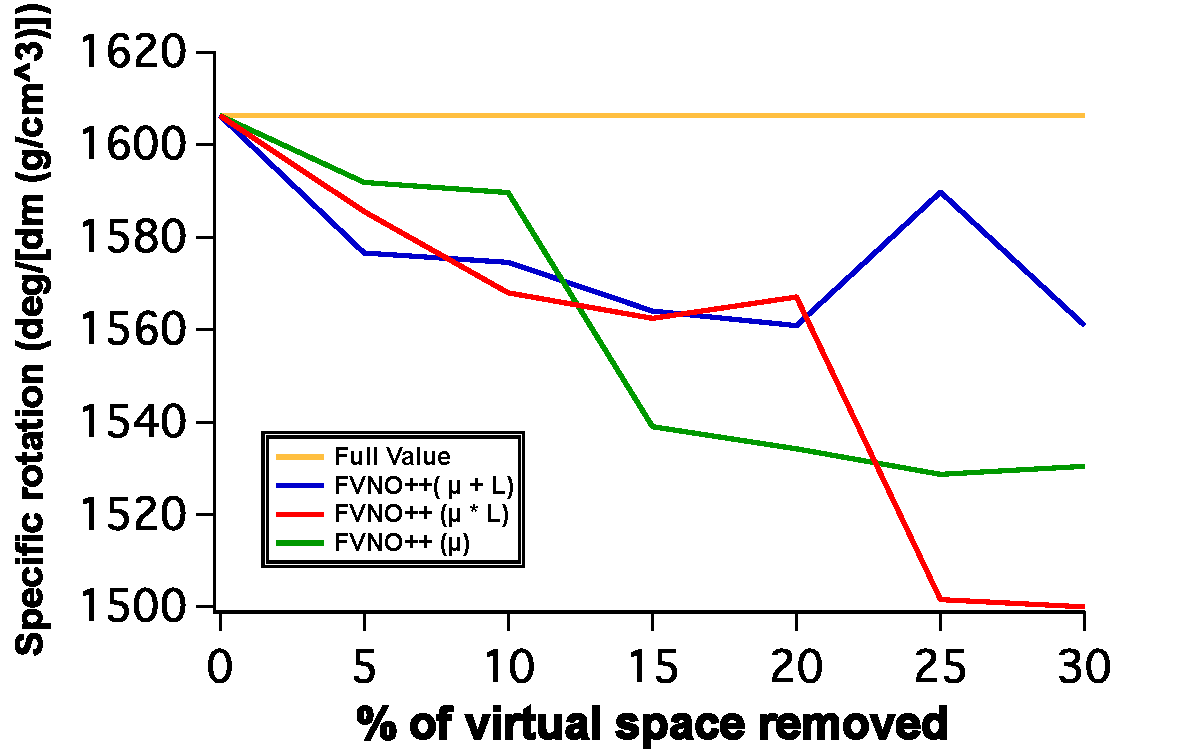
\includegraphics[width=0.6\linewidth]{figures_fvno++/fvno++_optrot_2_approaches}
\caption{{\footnotesize CCSD/aDZ specific rotations of
(H$_2$)$_7$ molecule in both FVNO++ ($\mu * L$) and FVNO++ ($\mu,L$) schemes as a function of
percentage of virtual space removed.}}
\label{fig:fvno++_optrot_2_approaches}
\end{MyFigure}
It can be seen that both the approaches start performing better than the FVNO++ ($\mu$) approach 
after a truncation of 10\% and yield similar results till about 20\% of the virtual space is removed.
However, the errors in the FVNO++ ($\mu * L$) method increase steeply threafter. Even though 
the FVNO++ ($\mu,L$) method yields the lowest errors out of all the three approaches, more
calculations are needed in order to confirm this behavior.
%for large-scale calculations. Moreover, the metric of retention might
%be not well-defined. Thus, we instead look at the performance
%of the second-order perturbed density approach which we have named as FVNO++ 
%in the next sections.
%\subsection{$(H_2)_n$ Helices}
%- Linear structure, chiral, helical arrangement
%- best case for local correlation problems
%- small masses, high OR
%- Polariz, specific rotation (h2)4, (h2)5, (h2)6, (h2)7, maybe-bigger!! : LG, MVG, aDZ basis
%- diagnostics for FVNO++ approach:
%	- first comparing the structure of the ground state and perturbed density, one can see 
%	  that perturbed density would have a higher rank than ground-state density.
%	- how about incorporating L*L density as well and optimized NOs by better guess densities.
%	- Here we mostly concentrate on capturing the right kind of behavior rather 
%  	than savings, since there is not enough sparsity on offer for these cases.
%  	This is applicable for other test cases as well.

%\subsection{beta-pinene}
%\subsection{phenyl-ethanol}
%\subsection{norbornenone}
%Maybe bring MP2 diagnostics here as a reason for poor behavior! I mean here the pi-pi*
%excitations might require accurate T2 amplitudes as well.
%\subsection{Sparsity in solvated cluster}
\section{Conclusions}
We propose a novel modification of the FVNO scheme for calculating linear
response properties at CC level of theory. The new scheme, which we have named
as FVNO++ constructs second-order perturbed densities to obtain ``perturbation
aware" VNOs whose ONs can be seen as a metric for estimating 
their importance in capturing the response of the wavefunction to the external 
perturbation. Based on plot studies on linear chiral molecules like H$_2$O$_2$ 
and (H$_2$)$_n$ helices, we conclude that this approach offers a very compact 
virtual space for calculating both dynamic polarizabilities and specific rotations
while maintaining very low truncation errors. However, more calculations are 
needed on two and three dimensional molecular systems to make the FVNO++ truncation 
scheme truly robust. We are currently in the process of implementing a RI-CC2 linear 
response code\cite{Friese12} which we intend to use in conjunction with the FVNO++ formalism 
to tackle large solvated clusters. Furthermore, we propose to extend this approach 
to the reduced-scaling domain based on pair natural orbitals\cite{Neese09,NeeseCCSD09}.
%- Within the FVNO++ formalism, explored structures of second-order perturbed densities:
%Dab(2)(MU), Dab(2)(P), Dab(2)(MU,L), Dab2(P,L), Dab(2)(L) 
%employing different guesses of first-order perturbed amplitudes.  
%Based on plot studies on h2o2, we can conclude that 
%this approach works, has the right behavior/convergence properties.
%however, as usual, specific rotation is more sensitive than
%polarizabilities %and requires bigger virtual spaces.
%Future work: We also wish to report the sparsity pattern of the guess densities of large
%solvated molecular clusters using DF-MP2 which give us an estimate of
%the computational savings that can be exploited for such systems.
%Real application is solvated clusters, where we conclude that
%Hopefully, there is a lot of sparsity to take advantage of.
%\section{Acknowledgements}

